\documentclass{book}
% -*- coding: utf-8 -*-

\usepackage[utf8x]{inputenc}
\usepackage{ucs}
\usepackage{lmodern}
\usepackage{graphicx}
\usepackage[frenchb]{babel}
\usepackage{hyperref,wrapfig}
\usepackage{amssymb}
\usepackage{latexsym}

\PrerenderUnicode{É} % Pre-render some accented chars for titles of chapter
\PrerenderUnicode{À}

\newcommand{\nop}{}

\begin{document}

%% uicilibris: begin 'Page de couverture'
\begin{titlepage}{\Large expEYES}\\[6em]
\begin{center}\includegraphics[width=1.0\textwidth]{eyes.jpg}\\[1em]
{\large Experiments for Young Engineers and Scientists}\\[6em]
{\Huge Manuel de l'utilisateur}\\[1em]
{\Large avec 50 Expériences Scientifiques}\\[3em]
\end{center}{\large Projet PHOENIXInter-University Accelerator Centre(A Research Centre of UGC) New Delhi 110 067 \href{http://www.iuac.res.in }{\mbox{http://www.iuac.res.in} }}\\
\end{titlepage}\pagebreak \tableofcontents \listoffigures\pagebreak






%% uicilibris: end 'Page de couverture' tables OK



%% uicilibris: begin 'Préambule'
\textbf{Préface}






Le projet PHOENIX (Physics with Home-made Equipment \&amp; Innovative Experiments) a commencé en 2004 au Inter-University Accelerator Centre avec l'objectif d'améliorer l'enseignement des sciences dans les Universités Indiennes. Le développement d'équipements de laboratoire à bas prix et la formation des professeurs sont les deux activités majeures de ce projet. Le premier produit était une interface généraliste, s'appelait aussi Phoenix, et s'articulait avec ces instruments tels qu'un compteur Geiger-Muller, un spectromètre alpha, etc. La puissance des ordinateurs personnels a été utilisée pour réaliser des expériences et de l'analyse de données. La conception du matériel est ouverte et le logiciel est publié sous la Licence Publique Générale GNU GPL. Les retours et le soutien de la communauté d'utilisateurs ont été cruciaux pour ce projet.



Le nouveau produit, expEYES (Experiments for Young Engineers \&amp; Scientists), est conçu pour être un outil pour étudier par l'expérimentation, valide pour les classes de collège et au-delà. On a essayé de maintenir un équilibre entre les expériences ouvertes principalement réservées à l'exploration et les expériences conventionnelles avec un objectif spécifique. Nous avons essayé d'optimiser la conception pour rester simple, souple, robuste et surtout bon marché. Il n'y a pas besoin d'une alimentation séparée, puisqu'il fonctionne à l'aide de l'alimentation 5V de la prise USB, indépendamment des pannes de courant communes à certains endroits. Le prix très abordable le rend accessible à des individus et nous espérons voir des étudiants faire des expériences hors des quatre murs du laboratoire, qui ferme quand sonne la cloche.



Vous pourrez trouver plus de détails et des versions mises à jour de ce document sur le site web \href{http://expeyes.in
 }{\mbox{http://expeyes.in
} }








Ajith Kumar



V V V Satyanarayana



Jimson Sacharias



Deepak Munda



S. Venkataramanan



(traduction française : Georges Khaznadar)









%% uicilibris: end 'Préambule' tables OK



%% uicilibris: begin 'Un bon départ'

\chapter{Un bon départ}



\section{Introduction}


On mesure plus souvent la performance d'un étudiant par sa capacité à mémoriser que par sa compréhension réelle. Le résultat est que la plupart échouent à appliquer ce qu'ils apprennent en classe aux choses qu'ils rencontrent dans la vie quotidienne. On peut corriger ça dans une certaine mesure par un enseignement basé sur l'exploration et l'expérience. En général, les expériences impliquent de contrôler quelques paramètres physiques tels que la température, la pression, la vitesse, l'accélération, la force, la tension, le courant, etc. Si la grandeur physique mesurée change rapidement, les mesures demandent à être automatisées et un ordinateur devient un outil utile. Par exemple, comprendre les variations du courant alternatif du secteur avec le temps nécessite de le mesurer toutes les millisecondes.



La possibilité de réaliser des expériences avec une précision raisonnable ouvre un champ entièrement nouveau dans l'enseignement de la science. Les étudiants peuvent comparer les données expérimentales avec les modèles mathématiques et examiner les lois fondamentales gouvernant des phénomènes variés. Les chercheurs formulent des hypothèses, conçoivent et réalisent des expériences, analysent les données pour vérifier si elles ont en accord avec la théorie. Les objectifs du projet PHOENIX (Physics with Home-made Equipment and Innovative Experiments) est de fournir les mêmes facilités aux étudiants à une échelle plus petite. On a déjà développé plusieurs équipements et expériences à ce jour. Ce document décrit quelques expériences qu'on peut faire avec l'interface nommée \emph{expEYES}.

\section{Le matériel : connexions externes}





\begin{figure}[h!]
\begin{center}
\caption{Le tableau de bord d'ExpEYES avec les connexions externes des deux côtés. Les flèches indiquent les sens des signaux. \label{fig:ExpEYES-top-panel}}\vspace{0.5em}
\includegraphics{top-panelcolor.png}
\end{center}
\end{figure}






Une photographie du matériel est présentée dans la figure  \ref{fig:ExpEYES-top-panel}. On peut le connecter au port USB d'un ordinateur. Il a 32 bornes d'entrée/Sortie, où on peut connecter des signaux du monde extérieur. Gardez en mémoire qu'il ne peut traiter que des signaux électriques, on peut suivre et contrôler les niveaux de tension à plusieurs bornes. Pour mesurer d'autre paramètres (tels que la température, la pression, etc.), il faut les convertir en signaux électriques en utilisant des éléments capteurs appropriés. Même si notre objectif premier est de faire des expériences, vous êtes encouragé à lire la brève description du matériel donnée ci-dessous.



\textbf{IMPORTANT} : \emph{Les tensions externes connectées à expEYES doivent être dans l'intervalle $\pm{}5\ V$}.




\subsection{Signaux numériques}


On peut groupe les connexions externes selon leurs fonctions.




\subsubsection{Entrées numériques (ID0 et ID1)}


Le logiciel peut lire le niveau de tension appliqué à ces bornes. Toute tension inférieure à 0,8 V est traitée comm 0 (BAS) et tout ce qui dépasse 2 V est traité comme 1 (HAUT). Si la tension change entres HAUT et BAS, ces bornes peuvent mesurer la fréquence et le rapport cyclique des signaux connectés. ExpEYES peut mesurer l'intervalle de temps entre les transitions de tension sur ces bornes avec une résolution de l'ordre de la microseconde.




\subsubsection{Sorties numériques (OD0 et OD1)}





à l'aide du logiciel, on peut commander la tension de ces bornes à 0 ou 5 V. OD0 est amplifiée par un transistor et peut contrôler un courant jusqu'à 100 mA. OD1 ne peut contrôler que jusqu'à 5 mA.




\subsection{Générateurs de signaux}






\subsubsection{SINE}





Générateur de signal sinusoïdal de fréquence fixe, la fréquence vaut environ 90 Hz. Sortie bipolaire avec une amplitude proche de 4 V.




\subsubsection{SQR1}





Peut générer un signal carré, oscillant entre 0 et 5 V La fréquence est programmable de 15 Hz à 1 MHz. Les valeurs de fréquences intermédiaires ne sont pas toutes possibles.




\subsubsection{SQR2}





Peut générer un signal carré, oscillant entre 0 et 5 V La fréquence peut être réglée à toute valeur entre 0,7 Hz et 90 kHz. L'oscillateur nécessite une résistance variable de $22\, k\Omega$ pour fonctionner. L'intervalle de fréquence est contrôlé par logiciel et le réglage fin de fréquence est fait en ajustant la résistance variable. Les intervalles de fréquence sont $< 25 Hz$, $25$ à $1 kHz$, $1 kHz$ à $10 kHz$ et $10 kHz$ à $90 kHz$. Quand on écrit une fréquence dans un intervalle particulier, ça choisit cet intervalle. On ajuste alors la résistance variable pour obtenir la fréquences désirée. La valeur réelle de la fréquence est mesurée et affichée durant l'ajustement.




\subsubsection{PULSE}





La fréquence de sortie est 488 Hz. Le rapport cyclique peut être programmé de 0 à 100 \%{} en 255 étapes. Cette borne peut être configurée pour générer un signal carré, comme SQR1. Cette propriété est utilisée par le programme qui démontre les interférences sonores.




\subsection{Entrées de tension analogiques}






\subsubsection{A0 et A1}





peuvent mesurer la tension dans un intervalle$\pm5\, V$ . La résolution de la conversion analogique-numérique est 12 bits. La tension à ces bornes peut être affichée en fonction du temps, ce qui donne la propriété d'un oscilloscope basse fréquence à deux canaux.




\subsubsection{A2}





Pour la mesure de tensions. L'entrée doit être dans un intervalle de 0 à 5 V. La résolution est de 12 bits. La tension peut être représentée en fonction du temps à l'aide du logiciel.




\subsection{Sorties de tension analogique}






\subsubsection{BPV}





Sortie de tension bipolaire. Peut être programmée à toute valeur entre -5 V et +5 V. La résolution est de 12 bits, ce qui implique un échelon de tension minimal de 2,5 mV.




\subsubsection{UPV}





Sortie de tension unipolaire. Peut être programmée entre 0 et +5 V. Ne peut pas être utilisée en même temps que la sortie de courant constant CS, dans la mesure où elles utilisent la même sortie de convertisseur numérique-analogique.




\subsubsection{IV}





Il s'agit juste de la sortie de BPV à travers une résistance de$1\, k\Omega$ . Utilisée pour faire des caractéristiques I-U.




\subsubsection{Source de courant constant (CS)}





programmable à toute valeur entre 0,05 et 2,0 mA. La résistance de charge devrait être choisie de telle façon que le produit $RI$  soit moins de 2 V. N'oubliez pas que CS et UPV partagent la même sortie de convertisseur numérique-analogique.




\subsection{Amplificateurs inverseurs}





Il y a trois amplificateurs inverseurs, implémentés à l'aide d'ampli-ops TLO84, désignés ci-dessous à l'aide de leurs numéros des bornes d'entrée et de sortie.




\subsubsection{15 $\Rightarrow$ 13}





Entrée à la borne 15 est sortie à la borne 13. Le gain par défaut est 50. On peut réduire le gain en mettant une résistance en série avec l'entrée. Le gain est donné par la relation $G=\frac{R_{f}}{(R_{ext}+1000)}$  où la résistance interne $R_{f}=50\,000\,\Omega$ . La résistance externe en série est $R_{ext}$ .




\subsubsection{14 $\Rightarrow$ 12}





Entrée à la borne 14 et sortie à la 12. Similaire au précédent.




\subsubsection{17 $\Rightarrow$ 18}





Entrée en 17 et sortie en 18. Le gain par défaut est 100. On peut réduire le gain en mettant une résistance en série avec l'entrée. Le gain est donné par la relation $G=\frac{R_{f}}{(R_{ext}+100)}$  où la résistance interne est $R_{f}=10\,000\,\Omega$  et la résistance externe en série est $R_{ext}$ .




\subsubsection{Amplificateur non-inverseur}





L'entrée est en 21 et la sortie en 22. Le gain est régi par une résistance externe $R_{g}$  connectée entre 19 et 20, et donné par la relation $Gain=1+10000/R_{g}$ . Cet amplificateur est implémenté à l'aide d'un circuit intégré OP27 et a une tension de décalage d'environ $30\,\mu V$.







\subsubsection{Entrée de capteur (SEN)}





Pour y connecter tout capteur dont la résistance varie avec le paramètre mesuré. Quand on l'utilise avec le photo-transistor, on branche le collecteur ici, et l'émetteur à la masse [Ground]. Capable de mesurer la tension et la fréquence.




\subsection{Fréquencemètres}





La borne 15 peut servir à mesurer la fréquence d'un signal bipolaire (qui varie entre des valeurs négatives et positives). L'amplitude minimale mesurable est 100 mV et la maximale est 5 V.



ID0, ID1 et SEN peuvent être utilisées pour mesurer la fréquence de signaux qui oscillent entre 0 et 5 V.




\subsection{Masses [Ground]}





Les bornes marquées GND et décorées d'un symbole de masse électrique représentent le niveau de tension 0 V. Elles sont connectées entre elles et à la masse de l'ordinateur à travers le câble USB.




\subsection{Comment connecter les fils}





On connecte les fils aux bornes à l'aide d'un tournevis. Desserrer la vis (la monter presque jusqu'en haut du connecteur), entrer le fil sur le côté et le serrer. On ne doit pas insérer les fils quand la vis est dans la position serrée. N'utiliser que le petit tournevis qui vient avec le kit. Quand on doit changer le connexion à une borne plusieurs fois durant une expérience, il sera commode de fixer une pince crocodile à cette borne.




\section{Installation du logiciel}





ExpEYES ne peut fonctionner que sur des ordinateurs ayant un interpréteur Python et un module Python pour accéder au port série USB. L'interface USB est gérée par des pilotes qui représentent le port USB comme un port série RS232 aux programmes de l'application. La communication avec expEYES est faite à l'aide d'une bibliothèque écrite en langage Python. Des programmes avec une interface utilisateur graphique ont été écrits pour plusieurs expériences. Il y de nombreuses façons de faire fonctionner le logiciel :




\subsection{Le CD vif expEYES}


la façon la plus simple pour commencer est de démarrer votre PC à l'aide du CD vif Phœnix. Dans le BIOS du PC, faites en sorte que le lecteur de CD soit le premier au démarrage, insérez le CD et redémarrez l'ordinateur. Un bureau apparaîtra et on peut démarrer expEYES depuis le menu  \texttt{\textbf{Applications -\&gt; Science}\nop}. Le CD vif expEYES est basé sur la distribution GNU/Linux Ubuntu 10.10.




\subsection{Installation dans une distribution GNU/Linux Debian ou Ubuntu}





Installer python-imaging-tk depuis le dépôt de la distribution qu'on a. Télécharger <code\&gt;expeyes.deb</code\&gt; depuis \href{http://expeyes.in }{\mbox{http://expeyes.in} } et l'installer. Installer aussi \emph{python-scipy} et \emph{grace} (un grapheur 2D) pour une pleine fonctionnalité.




\subsection{Pour les autres distributions GNU/Linux}





Télécharger <code\&gt;expeyes.tgz</code\&gt; depuis \href{http://expeyes.in }{\mbox{http://expeyes.in} } et suivre les instructions du fichier README. Il est important d’accorder des permissions de lecture/écriture à tous les utilisateurs sur le port USB où expEYES est connecté.




\subsection{Sous MSWindows}





Bien qu'expEYES soit un Logiciel Libre développé à l'aide de logiciels libres, il fonctionne sur des plateformes non-libres aussi. Pour l'installer sous MS Windows, il vous faut les fichiers suivants (donnés sur le CD) :
\begin{itemize}
  \item CDM20814\_Setup.exe
  \item python-2.6.6.msi
  \item pyserial-2.5.win32.exe
  \item PIL-1.1.7.win32-py2.6.exe
  \item numpy-1.6.0b2-win32-superpack-python2.6.exe
  \item scipy-0.9.0-win32-superpack-python2.6.exe
  \item expeyes.zip
\end{itemize}



Dézipper le fichier <code\&gt;expeyes.zip</code\&gt;, cliquer double sur <code\&gt;explore.py</code\&gt; dans le répertoire nommé EYES nouvellement créé.



Si vous avez le CD vif nommé \textbf{expEYES}, examinez le contenu du dossier nommé WINEYES. Tous les fichiers mentionnés ci-dessus sont dans ce dossier. Cliquez double sur eux dans l’ordre mentionné ci-dessus pour les installer. L'utilitaire grapheur XmGrace n'est pas disponible sous Windows. La sortie de la transformée de Fourier sera enregistrée sur le disque au format texte.




\section{Le programme graphique principal}


Lancez  \texttt{\textbf{Applications-\&gt;Science-\&gt;expEYES}\nop} depuis le menu. Ça lance une fenêtre graphique comme dans la figure  \ref{fig:Explorer-screenshot}, voyez l'explication ci-dessous.
\begin{itemize}
  \item Un clic sur les boîtes où s'affichent les numéros de bornes permet d'accéder à de l'aide en ligne.
  \item Le statut des entrées numériques décide de la couleur de la zone juste à côté d'elles. Un vert pâle signifie HAUT et un gris signifie BAS. Quand on applique une tension oscillant entre 0 et 5V, ce champ va clignoter.
  \item La zone d'affichage près de la borne 15 peut clignoter si un signal alternatif est connecté là.
  \item La zone d'affichage de la fréquence de SEN peut clignoter si la tension d'entrée varie entre 0 et 5 V.
  \item Les boutons marqués « F » peuvent être utilisés pour mesurer la fréquence, quand les champs colorés sont en train de clignoter.
  \item On peut fixer la valeur des signaux de sortie en les entrant dans la boîte de texte voisine. On peut fixer la tension, le courant, la fréquence et le rapport cyclique de cette façon. Tapez  \fbox{Entrée} pour rendre la valeur effective. En cas de succès, un point décimal sera affiché.
  \item SQR2 nécessite la résistance externe de $22\, k\Omega$  pour fonctionner. La fréquence réelle est affichée juste sous le champ texte, là où on fixe la fréquence.
  \item Les états des sorties numériques, OD0 et OD1, peuvent être changés en utilisant les boutons à cocher.
  \item Les tensions aux bornes d'entrées 23, 24, 25 et 26 sont affichées constamment à côté d'elles.
\end{itemize}




\subsection{La fenêtre du graphique}





La fenêtre de graphique à droite fonctionne comme un oscilloscope à basse fréquence. La cadence d'échantillonnage maximale est de 100 kHz seulement. On peut numériser des signaux sinusoïdaux en utilisant un seul canal jusqu'à 20 kHz, et jusqu'à 10 kHz quand les deux canaux sont utilisés. Les contrôles suivants sont disponibles :



\begin{itemize}
  \item Curseur d'échelle horizontale (ms/carreau). Le mettre à la valeur minimale puis augmenter pour voir plus de périodes à l'écran.
  \item Cases à cocher pour sélectionner A0 et A1.
  \item Case à cocher LIZ pour faire une figure de Lissajous à l'aide des entrées A0 et A1.
  \item Case à cocher FIT pour activer le calcul de l'amplitude, de la fréquence et de la phase en modélisant [to fit] les données à l'aide de l'équation $V=V_{0}\sin\left(\omega t+\theta\right)+C$.
  \item Bouton SAVE pour enregistrer les données dans le fichier <code\&gt;explore.dat</code\&gt; (format : deux colonnes de texte).
  \item FT pour calculer un spectre de puissance par transformation de Fourier [Fourier Transform] des données des canaux activés. Si XmGrace et pygrace sont installés, une fenêtre s'ouvre. Le spectre de puissance est enregistré dans le fichier <code\&gt;exploreFFT.dat</code\&gt; en format texte.
\end{itemize}




\section{Mesures élémentaires à l'aide d'expEYES}





\begin{figure}[h!]
\begin{center}
\caption{Copie d'écran du programme Explore. Les flèches indiquent la direction des signaux. Les champs textes servent à fixer des valeurs. Des boutons sont fournis pour les mesures de fréquences. \label{fig:Explorer-screenshot}}\vspace{0.5em}
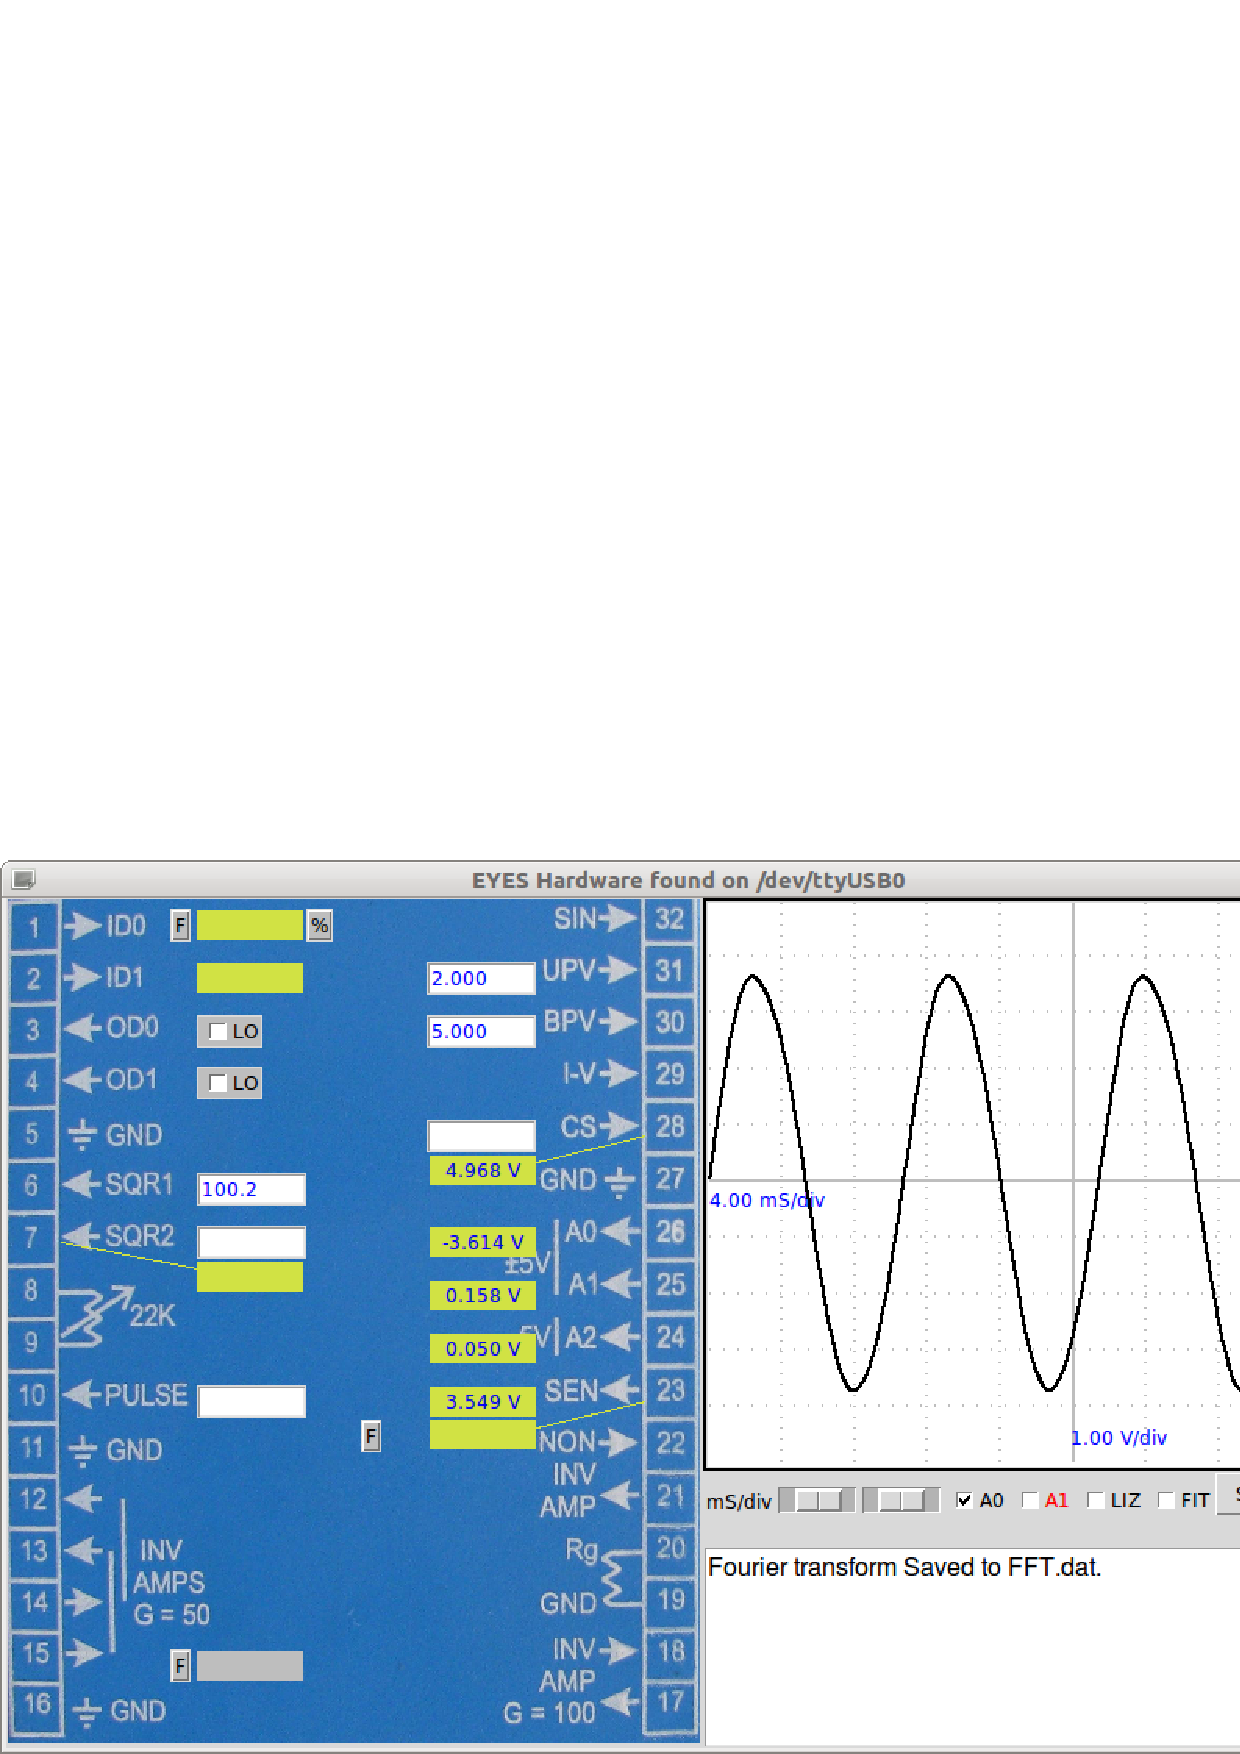
\includegraphics[width=0.95\textwidth]{explorer.png}
\end{center}
\end{figure}



Avant de commencer les expériences, faisons quelques exercices simples pour nous familiariser avec ExpEYES. Démarrez votre ordinateur avec le cédérom vif, connectez ExpEYES au port USB et démarrez le programme ExpEYES depuis le menu  \texttt{\textbf{Applications-\&gt;Science}\nop}.




\subsection{Générer \&amp; mesurer des tensions}


\begin{itemize}
  \item Connecter BPV à A0
  \item Fixer BPV à une certaine tension et observer l'affichage à A0
  \item Essayer A1 au lieu de A0
  \item Répéter la même chose en connectant UPV à A2
\end{itemize}




\subsection{Observer des signaux de tension}





\begin{itemize}
  \item Connecter SQR1 à A0
  \item Fixer SQR1 à 100 Hz
  \item Ajuster l'échelle horizontale (ms/Div) pour voir 4 ou 5 périodes du signal carré
  \item Répéter la même chose avec d'autres valeurs de fréquence
  \item Connecter SINE à A1 et observer les deux traces simultanément
  \item Explorez les option FIT, XM et FT.
\end{itemize}




\subsection{Mesurer la fréquence}





\begin{itemize}
  \item Connecter SQR1 à ID0
  \item Fixer SQR1 à 1000
  \item Cliquer sur le bouton « F » de ID0
  \item Connecter SINE à la borne 15 et mesurer la fréquence\footnote{La borne 15 ne peut pas mesurer la fréquence des sorties SQR1 ou SQR2, parce qu'elles n'oscillent pas en-dessous de zéro.}.
\end{itemize}

\subsection{Mesurer le Connecter PULSE à ID0}





\begin{itemize}
  \item Connecter aussi à A0, si on veut observer la forme du signal.
  \item Fixer PULSE à une valeur quelconque comprise entre 0 et 100
  \item Cliquer sur le bouton « \%{} » de ID0, pour mesurer le rapport cyclique.rapport cyclique
\end{itemize}




\subsection{Fixer des niveaux de tension}





\begin{itemize}
  \item Connecter OD0 à ID0
  \item Cliquer sur le bouton à cocher observer la couleur d'affichage de ID0.
\end{itemize}










\section{Expériences}


Une expérience scientifique implique en général le contrôle et la mesure de divers paramètres physiques comme la température, la pression, la tension, le courant, etc. Le matériel de base d'expEYES peut générer différentes sortes de signaux électriques et mesurer des signaux électriques. Pour mesure quoi que ce soit d'autre qu’une tension, il faut convertir à l'aide d'éléments capteurs appropriés. Par exemple un capteur de température donnera une tension indiquent la température. Comme les expériences en électricité et magnétisme ne nécessitent aucun capteur, nous avons plus d'expériences basées sur l'électricité et le magnétisme.



Un programme avec une interface graphique est fourni pour chacune des expériences de ce manuel. Cependant il est possible de faire la même chose en écrivant quelques lignes en langage Python. Toute la communication avec expEYES est faite à l'aide d'une bibliothèque Python nommée <code\&gt;eyes.py</code\&gt;. Des bibliothèques Python sont utilisées pour l'analyse des données. Si vous êtes intéressé par développer de nouvelles expériences basées sur expEYES, c'est une bonne idée d'étudier le langage de programmation Python. Pratiquement chaque expérience peut être étendue d'une façon ou d'une autre et quelques suggestions sont faites dans ce sens.



Les chapitres suivants décrivent des expériences sur divers sujets comme l'électricité, le magnétisme, l'électronique, le son, la chaleur, etc. Comme le kit expEYES est destiné à l'auto-apprentissage, nous avons inclus quelques expériences très triviales au début.



%% uicilibris: end 'Un bon départ' tables OK



%% uicilibris: begin 'Expériences'

\chapter{Expériences}





Nous commençons avec la tâche triviale de mesurer la tension d'une pile. On introduit ensuite le courant et la résistance, puis des résistances changeant avec la lumière et la température. Le concept de Courant Alternatif est introduit en traçant le graphique d'une tension en fonction du temps.



Le comportement d'éléments de circuit comme des condensateurs et des bobinages en courant alternatif et continu sont explorés, en mesurant des paramètres tels que l'amplitude, la fréquence et la phase. La réponse transitoire d'une résistance et d'un condensateur en série est utilisée pour mesurer la capacité. L'inductance est aussi mesurée de cette façon. On examine l'effet de matériaux ferromagnétiques dans un bobinage.



L'analyse de Fourier d'un signal carré est faite pour étudier les harmoniques. L'intégration et la différentiation d'un signal carré à l'aide de circuits RC est aussi explorée.



%% uicilibris: end 'Expériences' tables OK



%% uicilibris: begin 'Mesurer la tension'

\section{Mesurer la tension}



\subsection{Objectif}


Apprendre à mesurer la tension à l'aide d'expEYES et acquérir une notion du concept de masse électrique [Electrical Ground].




\subsection{Matériel}


\begin{figure}[h!]
\begin{center}
\caption{\label{measuring-drycells}Mesure de la tension de piles sèches }\vspace{0.5em}
\includegraphics[width=0.4\textwidth, height=0.3\textwidth, keepaspectratio]{Schematic-cell-voltage.png}
\includegraphics[width=0.4\textwidth, height=0.3\textwidth, keepaspectratio]{Pic-drycell-voltage.png}
\end{center}
\end{figure}



\begin{itemize}
  \item piles sèches de tensions 1,5 V
  \item Support de piles avec deux fils de connexion.
\end{itemize}

\subsection{Procédure}


\begin{itemize}
  \item Connecter le Négatif de la pile sèche à la masse [Ground].
  \item Borne positive de la pile en A0.
\end{itemize}

\subsection{Observation}


La tension sera affichée à gauche de A0, comme montré sur la figure \ref{measuring-drycells}.

\subsection{Discussion}


On mesure la différence de potentiel expEYES mesurent la tension par rapport aux bornes de masse marquées GND. Nous avons connecté la borne négative de la pile à la masse [Ground]. La borne positive est à +3 V par rapport à la borne négative.



Recommencer l'expérience en connectant la borne positive de la pile à GND et la négative à A0. La tension sera présentée comme négative. \emph{Est-ce que ça donnerait la tension correcte, si la masse [Ground] n'était pas connectée ?}



%% uicilibris: end 'Mesurer la tension' tables OK



%% uicilibris: begin 'Tension, courant et résistance'

\section{Tension, courant et résistance}



\subsection{Objectif}


En apprendre au sujet du courant, de la résistance, et de la loi d'Ohm. Tracer la courbe courant-tension [I-V] d'une résistance.

\subsection{Théorie}


La tension aux bornes d'un conducteur est directement proportionnelle au courant qui le traverse. La constante de proportionnalité est nommée Résistance. Ceci est connu sous le nom de Loi d'Ohm, avec l'expression mathématique suivante :



$U\varpropto I\,\,\,;\,\,\,\, U=RI\,\,\,\, ou\,\,\, R=\frac{U}{I}$

\subsection{Matériel}


\begin{figure}[h!]
\begin{center}
\caption{\label{fig:I-V-of-resistor}Caractéristique I-V d'une résistance }\vspace{0.5em}
\includegraphics[width=0.4\textwidth, height=0.3\textwidth, keepaspectratio]{Schematic-res-measure.png}
\includegraphics[width=0.4\textwidth, height=0.3\textwidth, keepaspectratio]{Pic-resistor-iv.png}
\end{center}
\end{figure}



\begin{itemize}
  \item Une résistance de $1 k\Omega$
\end{itemize}

\subsection{Procédure}


\begin{itemize}
  \item Connecter la résistance entre la source de courant CS et la masse [Ground].
  \item Fixer le courant à 0,5 mA et noter la tension en CS.
  \item Changer le courant par paliers de 0,5 mA. (La tension ne devrait pas dépasser 2 V à la borne CS)
  \item Faire un clic droit sur le tableau de bord. Choisir  \texttt{\textbf{Resistor IV}\nop} dans le menu contextuel.
  \item Tracer le graphique à l'aide du bouton  \fbox{START}.
\end{itemize}

\subsection{Observation}


\begin{tabular}{|l|l|}
\hline
\textbf{I (mA)}&\textbf{U (V)}
\\ \hline
0,5&0,508
\\ \hline
1,0&1,011
\\ \hline
1,5&1,510
\\ \hline
\end{tabular}\\[0.5em]






La précision de la source de courant n'est que de 1\%{}, à cause de la tolérance sur la valeur de la résistance utilisée. Pour les applications nécessitant une précision supérieure, on peut la calibrer à l'aide d'une résistance connue. La courbe I-V est présentée à la figure  \ref{fig:I-V-of-resistor}.

\subsection{Discussion}


À l'aide d'expEYES, on peut fixer le courant issu de CS (de 0,05 mA à 2 mA). La tension en CS dépend de la résistance connectée de la source de courant à la masse [Ground]\footnote{La tension aux bornes de cette source de courant particulière ne devrait pas dépasser 2 V. Choisir la résistance de charge et les valeurs de courant en fonction de ça.}.La tension aux bornes de cette source de courant particulière ne devrait pas dépasser 2 V. Choisir la résistance de charge et les valeurs de courant en fonction de ça.



Le graphique est une ligne droite comme la tension est directement proportionnelle au courant. La courbe ne sera pas une ligne droite pour les éléments non-linéaires, comme une diode.






%% uicilibris: end 'Tension, courant et résistance' tables OK



%% uicilibris: begin 'Résistances en série'

\section{Résistances en série}



\subsection{Objectif}


Trouver la résistance équivalente à une combinaison en série de résistances.

\subsection{Théorie}


Pour les combinaisons en série de résistances, la résistance totale est donnée par $R=R1+R2+\cdots$

\subsection{Matériel}


Résistances de $560\,\Omega$  et $1\, k\Omega$.

\subsection{Procédure}


\begin{figure}[h!]
\begin{center}
\includegraphics[width=0.4\textwidth, height=0.3\textwidth, keepaspectratio]{Schematic-res-series.png}
\end{center}
\end{figure}



Connecter les deux résistances en série entre CS et la masse [Ground]



Fixer le courant à 1 mA et prendre note de la tension affichée à la borne CS.

\subsection{Observation}


\begin{tabular}{|l|l|}
\hline
\textbf{R ($\Omega$)}&\textbf{U (V)}
\\ \hline
560&0,558
\\ \hline
1000&0,998
\\ \hline
1000+560&1,556
\\ \hline
\end{tabular}\\[0.5em]



Comme le courant est le même, la tension totale donne la résistance effective. On peut voir que c'est la somme des valeurs individuelles, dans la limite de l'erreur de mesure.

\subsection{Discussion}


Les très fortes résistances ($\&gt;10^{9}\Omega$) sont souvent réalisées à l'aide d'associations en série.



%% uicilibris: end 'Résistances en série' tables OK



%% uicilibris: begin 'Résistances en parallèle'

\section{Résistances en parallèle}



\subsection{Objectif}


Trouver la résistance équivalente à une association de résistances en parallèle.

\subsection{Théorie}


Pour les associations en parallèle, la résistances effective est donnée par la relation :



$\frac{1}{R}=\frac{1}{R1}+\frac{1}{R2}+\cdots$

\subsection{Matériel}


Deux résistances de 1k$\Omega$

\subsection{Procédure}


\begin{figure}[h!]
\begin{center}
\includegraphics[width=0.4\textwidth, height=0.3\textwidth, keepaspectratio]{Schematic-res-par.png}
\end{center}
\end{figure}



\begin{itemize}
  \item Connecter une résistances de 1 k$\Omega$  entre CS et la masse [Ground].
  \item Fixer le courant à 1 mA (0,001 A) et prendre note de la tension affichée à CS.
  \item Répéter la même chose avec deux résistances connectées en parallèle.
\end{itemize}

\subsection{Observation}


\begin{tabular}{|l|l|}
\hline
\textbf{$R_{connectee}(\Omega)$}&\textbf{$U_{mesuree}(V)$}
\\ \hline
1000&1,008
\\ \hline
1000 $\parallel$ 1000&0,503
\\ \hline
\end{tabular}\\[0.5em]
Comme nous connaissons le courant, à partir des tensions mesurées, nous pouvons calculer la résistance. Selon la tension mesurée la résistance de l'association en parallèle est $\frac{0.503\, V}{0.001\, A}=503\,\Omega$

\subsection{Discussion}


\emph{Pour quelles raisons voudrait-on connecter des résistances en parallèle ?}



%% uicilibris: end 'Résistances en parallèle' tables OK



%% uicilibris: begin 'Mesure de résistance par comparaison'

\section{Mesure de résistance par comparaison}


 \label{sec:Measure-resistance-by}

\subsection{Objectif}


Apprendre à appliquer la Loi d'Ohm pour trouver la valeur d'une résistance inconnue en la comparant avec une résistance connue.

\subsection{Théorie}


La tension aux bornes d'une résistance est donnée par $ U=RI$. Si le courant qui traverse deux résistances est le même, alors le quotient des tensions sera le même que le quotient des résistances.



$I=\frac{U_{1} }{R_{1} }=\frac{U_{2} }{R_{2} }$

\subsection{Matériel}


Une résistance de référence de 1 k$\Omega$  et quelques autres résistances. (valeurs entre 100 $\Omega$  et 10 k$\Omega$ )

\subsection{Procédure}


\begin{itemize}
  \item Connecter la résistance inconnue entre UPV et A2.\footnote{On utilise A2 quand la tension est comprise entre 0 et 5 V.}
  \item Connecter la résistance de 1 k$\Omega$  ($R_{2}$) entre A2 et la masse [Ground].
  \item Fixer UPV à 4 V.
  \item Mesurer la tension en A2.
\end{itemize}

\subsection{Observation}


La tension en A2 = 1,244 V, ce qui implique que la tension aux bornes de la résistance inconnue est $4-1,244=2,756V$



Le courant est $I=\frac{1,244}{1000}=1,244mA$



La valeur de la résistance inconnue est $R_1=\frac{2,756}{1,244}=2,215\, k\Omega$

\subsection{Discussion}


Quelle est la limite de cette méthode ? Comment choisit-on la résistance de référence ? supposons que la valeur inconnue soit en méga-ohm, quel serait la chute de tension dans une résistance de référence de 1 k$\Omega$ ? Notre mesure de tension possède une résolution de $\frac{1}{4095}$ .



Nous utiliserons cette méthode plus tard pour mesurer la résistance de solutions.






%% uicilibris: end 'Mesure de résistance par comparaison' tables OK



%% uicilibris: begin 'Tension d'une pile au citron'

\section{Tension d'une pile au citron}



\subsection{Objectif}


Créer une source de tension. En apprendre sur la possibilité de générer du courant. Concept de résistance interne.




\subsection{Matériel}


\begin{itemize}
  \item Un citron mur (ou un acide quelconque), des plaques fines de zinc et de cuivre.
  \item Une résistance de 1 k$\Omega$.
\end{itemize}

\subsection{Procédure}


\begin{figure}[h!]
\begin{center}
\caption{\label{fig:lemoncell}(a) des plaques de zinc et de cuivre insérées dans un citron. (b) La tension continue produite par la pile. }\vspace{0.5em}
\includegraphics[width=0.4\textwidth, height=0.3\textwidth, keepaspectratio]{Schematic-lemon-cell.png}
\includegraphics[width=0.4\textwidth, height=0.3\textwidth, keepaspectratio]{Pic-lemoncellDC.png}
\end{center}
\end{figure}



\begin{itemize}
  \item Insérer les plaques de zinc et de cuivre dans le citron.
  \item Connecter une plaque à la masse [Ground] et l'autre à A0, à l'aide de deux fils électriques.
  \item Connecter la résistance entre A0 et la masse [Ground].
\end{itemize}

\subsection{Observation}


La tension entre le cuivre et le zinc sera d'environ 0,9 V. Quand on connecte la résistance, celle-ci diminue jusqu'à environ 0,33 V.



Quelle est la résistance interne de la pile ?

\subsection{Discussion}


Quand la résistance est connectée, le courant commence à circuler par elle. Mais pourquoi la tension diminue-t-elle ?



Ça ne se produit pas avec une pile sèche neuve. Pourquoi ?



Le courant est causé par le mouvement de charges électriques et il doit faire le tour complet. Cela signifie que le courant doit traverser la pile aussi. Selon la résistance interne de la pile, une part de la tension est perdue à l'intérieur de la pile elle-même.



Une source de tension idéale devrait posséder une résistance interne nulle.



%% uicilibris: end 'Tension d'une pile au citron' tables OK



%% uicilibris: begin 'Tension variable dans le temps'

\section{Tension variable dans le temps}



\subsection{Objectif}


Introduire le concept de tensions dépendant du temps, à l'aide d'un graphique U(t).




\subsection{Matériel}


\begin{itemize}
  \item Piles sèches de tensions 1,5 V
  \item Support de piles avec fils de connexion.
\end{itemize}

\subsection{Procédure}


\begin{figure}[h!]
\begin{center}
\caption{\label{fig:Graph-of-DC}Graphique d'une tension continue en fonction du temps }\vspace{0.5em}
\includegraphics[width=0.4\textwidth, height=0.3\textwidth, keepaspectratio]{Schematic-cell-voltage.png}
\includegraphics[width=0.4\textwidth, height=0.3\textwidth, keepaspectratio]{Pic-dcvoltage.png}
\end{center}
\end{figure}



\begin{itemize}
  \item Connecter le négatif de la pile sèche à la masse [Ground].
  \item Borne positive de la pile en A0.
  \item Observer le graphique dans la partie droite de la fenêtre.
\end{itemize}

\subsection{Observation}


Une ligne horizontale apparaît sur le graphique, le temps est sur l'axe des abscisses et la tension est sur l'axe des ordonnées.

\subsection{Discussion}


La tension est constante dans le temps. Une pile est une source de tension continue. Un autre type de tension est nommé tension alternative, elle change de valeur et de signe dans le temps.



%% uicilibris: end 'Tension variable dans le temps' tables OK



%% uicilibris: begin 'Tension alternative'

\section{Tension alternative}



\subsection{Objectif}


En apprendre un peu au sujet de la tension alternative, à l'aide de graphiques. Se familiariser avec la forme d'onde sinusoïdale.




\subsection{Matériel}


\begin{itemize}
  \item Un bout de fil électrique.
\end{itemize}

\subsection{Procédure}


\begin{figure}[h!]
\begin{center}
\caption{\label{fig:Sinewave}Forme de l'onde de tension alternative issue de SIN }\vspace{0.5em}
\includegraphics[width=0.4\textwidth, height=0.3\textwidth, keepaspectratio]{Schematic-sine-a0.png}
\includegraphics[width=0.4\textwidth, height=0.3\textwidth, keepaspectratio]{Pic-sinewave90hz.png}
\end{center}
\end{figure}



\begin{itemize}
  \item Connecter SIN à A0.
  \item Ajuster l'échelle horizontale pour voir 4 ou 5 périodes.
  \item Activer la case à cocher  \fbox{FIT}.
\end{itemize}

\subsection{Observation}


La forme d'onde est montrée à la figure  \ref{fig:Sinewave}. Activer l'option  \fbox{FIT} pour calculer l'amplitude et la fréquence en modélisant les données à l'aide de l'équation $U=U_{0}\sin(2\pi ft+\theta)$, où $U_{0}$  est l'amplitude et $f$  est la fréquence.

\subsection{Discussion}


La tension change avec le temps. Elle devient tantôt positive tantôt négative. Une période complète dure environ 12 milli-secondes, c'est à dire environ 90 périodes par seconde ou 90 Hz. Cette forme d'onde de tension est générée par des circuits électroniques.\footnote{La fréquence de la sortie SIN est proche de 90 Hz. Ses variations sont dues à la tolérance de 20\%{} sur les valeurs des condensateurs qui décident de la fréquence.}



La tension d'alimentation du secteur dans nos maisons a une fréquence de 50 Hz.



Quelle est la signification de $\theta$ dans l'équation ci-dessus ?






%% uicilibris: end 'Tension alternative' tables OK



%% uicilibris: begin 'Influence d'une tension alternative'

\section{Influence d'une tension alternative}



\subsection{Objectif}


En apprendre un peu au sujet de la tension alternative du secteur. Explorer le phénomène de propagation de tensions alternatives à travers l'espace.




\subsection{Matériel}


\begin{itemize}
  \item Un bout de fil électrique long.
\end{itemize}

\subsection{Procédure}


\begin{figure}[h!]
\begin{center}
\caption{\label{fig:Power-line-pickup}Influence d'un câble électrique connecté au secteur }\vspace{0.5em}
\includegraphics[width=0.4\textwidth, height=0.3\textwidth, keepaspectratio]{Schematic-pickup.png}
\includegraphics[width=0.4\textwidth, height=0.3\textwidth, keepaspectratio]{Pic-sinewave50hz.png}
\end{center}
\end{figure}



\begin{itemize}
  \item Connecter une extrémité du fil électrique en A0.
  \item Placer l'autre extrémité du fil électrique près d'un câble électrique relié au secteur (ne jamais toucher le câble) et changer l'orientation du fil jusqu'au moment où on a un bon signal sur l'écran.
  \item Ajuster l'échelle horizontale à 10 milli-secondes par division.
  \item Activer la case à cocher« FIT ».
\end{itemize}

\subsection{Observation}


La forme de tension observée est montrée à la figure  \ref{fig:Power-line-pickup}. La fréquence calculée par modélisation des données est 49,65 Hz

\subsection{Discussion}


Sans réaliser aucun branchement, comment se fait-il qu'on récupère une tension alternative depuis le secteur ? Faire cette expérience avec un ordinateur portable situé loin des lignes de courant du secteur.



Est-ce similaire aux radiations d'un téléphone cellulaire ?



Pourquoi la fréquence diffère-t-elle de 50 Hz ?



Nous observons la tension reçue par influence par le fil électrique, qui agit comme un antenne captant la radiation à 50 Hz issue du câble du secteur. Quand on touche le bout flottant du fil électrique on augmente le signal, parce qu'on fait alors partie de l'antenne. La fréquence $f$  est calculée en modélisant les données recueillies par l'équation $U=U_{0}\sin(2\pi ft+\theta)$.



Essayez de faire les mesures durant la journée et à minuit pour comparer les fréquences mesurées. Elles dépendent de la charge du réseau électrique. Si la distribution de l'énergie électrique est vraiment bonne, la fréquence restera constante\footnote{N.d.T. :En Inde où ExpEYES a été conçu, les usines de production d'électricité cherchent à asservir la fréquence f à la valeur 50 Hz. Il y a donc toujours une petite différence entre la fréquence f et la valeur de référence 50 Hz. En Europe, les usines cherchent plutôt à asservir la phase $\theta\,$ en utilisant une source de fréquence commune (f=50 Hz). Cette dernière méthode donne une plus grande stabilité de la fréquence.}.






%% uicilibris: end 'Influence d'une tension alternative' tables OK



%% uicilibris: begin 'Composantes continue et alternative d'une tension'

\section{Composantes continue et alternative d'une tension}


  \label{sec:DC-AC}

\subsection{Objectif}


En apprendre un peu au sujet des composantes continue et alternative d'une tension dépendante du temps. Séparer les composantes continue et alternative à l'aide d'un condensateur.




\subsection{Matériel}


\begin{itemize}
  \item condensateur de $1 \mu{}F$, résistance de 10 k$\Omega$
\end{itemize}

\subsection{Procédure}


\begin{figure}[h!]
\begin{center}
\caption{\label{fig:Square-wave}(a) Tension oscillant entre 0 et 5 V }\vspace{0.5em}
\includegraphics[width=0.4\textwidth, height=0.3\textwidth, keepaspectratio]{Schematic-sqr-a0.png}
\includegraphics[width=0.4\textwidth, height=0.3\textwidth, keepaspectratio]{Pic-sqrwave2.png}
\end{center}
\end{figure}



\begin{figure}[h!]
\begin{center}
\caption{\label{}(b) Après traversée d'un condensateur }\vspace{0.5em}
\includegraphics[width=0.4\textwidth, height=0.3\textwidth, keepaspectratio]{Schematic-ac-dc.png}
\includegraphics[width=0.4\textwidth, height=0.3\textwidth, keepaspectratio]{Pic-sqrwave-dcblocked.png}
\end{center}
\end{figure}



\begin{itemize}
  \item Connecter SQR1 à A0 à l'aide d'un fil électrique.
  \item Entrer 500 dans la boîte texte de SQR1 et appuyer sur la touche <Entrée\&gt;.
  \item Ajuster l'échelle horizontale pour voir plusieurs périodes.
  \item Insérer un condensateur de 1 µF entre SQR1 et A0
  \item Connecter une résistance de 10 k$\Omega$  entre A0 et la masse [Ground].
\end{itemize}

\subsection{Observation}


Les formes d'ondes observées avec et sans le condensateur en série sont montrées à la figure  \ref{fig:Square-wave}. La tension oscille entre 0 et 5 V. Après avoir traversé le condensateur, la tension oscille entre -2,5 V et +2,5 V.

\subsection{Discussion}


Qu'obtiendrez-vous si vous faisiez la soustraction de 2,5 V de la coordonnée-y de chaque point du premier graphique ? C'est ce que le condensateur a réalisé. Il s'est opposé au passage de la composante en tension continue.



La tension d'origine peut être considérée comme la superposition de d'une tension alternative de 5 V (crête à crête) et d'une tension continue de 2,5 V.



Il se peut qu'on doive connecter une résistance de 10 k$\Omega$  entre A0 et la masse [Ground] pour voir un signal oscillant entre-2,5 et +2,5 V.



Pourquoi cette résistance est-elle nécessaire ?



%% uicilibris: end 'Composantes continue et alternative d'une tension' tables OK



%% uicilibris: begin 'Résistivité du corps humain'

\section{Résistance du corps humain}



\subsection{Objectif}


Avoir une idée de la résistance de la peau humaine, et savoir comment elle varie.




\subsection{Matériel}


\begin{itemize}
  \item Deux bouts de fil électrique.
\end{itemize}

\subsection{Procédure}


\begin{figure}[h!]
\begin{center}
\caption{\label{}Tension après passage dans la main. }\vspace{0.5em}
\includegraphics[width=0.4\textwidth, height=0.3\textwidth, keepaspectratio]{Schematic-cond-main.png}
\includegraphics[width=0.4\textwidth, height=0.3\textwidth, keepaspectratio]{Pic-sqrwave-hand.png}
\end{center}
\end{figure}



\begin{itemize}
  \item Connecter un bout d'un fil à SQR1, laisser l'autre bout en l'air
  \item Connecter un bout du second fil électrique à A0.
  \item Fixer SQR1 à 500.
  \item Ajuster l'échelle horizontale pour voir plusieurs périodes.
  \item Tenir les extrémités libres des fils électriques entre vos doigts.
  \item Répéter la même chose en utilisant SINE au lieu de SQR1.
\end{itemize}




\subsection{Discussion}


En utilisant la méthode de comparaison, essayez de calculer la résistance de la portion de main entre les deux fils, quand vous les tenez. La résistance de référence est $10 M\Omega$, connectée en interne entre A0 et la masse.



%% uicilibris: end 'Résistivité du corps humain' tables OK



%% uicilibris: begin 'Résistances dépendantes de la température'

\section{Résistances dépendantes de la température}



\subsection{Objectif}


Montrer la dépendance de la résistance en fonction d la température. Concept de base d'un capteur de température.




\subsection{Matériel}


\begin{itemize}
  \item Thermistance (NTC)\footnote{en anglais : Negative Temperature Coefficient}. Résistance $1\ k\Omega$  à 25° Celsius.
  \item De l'eau froide
  \item Une bougie ou une autre source de chaleur.
\end{itemize}

\subsection{Procédure}


\begin{figure}[h!]
\begin{center}
\caption{\label{} }\vspace{0.5em}
\includegraphics[width=0.4\textwidth, height=0.3\textwidth, keepaspectratio]{Schematic-ntc.png}
\end{center}
\end{figure}



\begin{itemize}
  \item Connecter la thermistance (NTC) entre CS et la masse [Ground]
  \item Fixer CS à $1,0\ mA$
  \item Mesurer la tension aux bornes de la thermistance à diverses températures.
\end{itemize}

\subsection{Observation}


\begin{tabular}{|l|l|l|}
\hline
\textbf{Réglage}&\textbf{$U=RI$}&\textbf{$R=\frac{U}{I}$}
\\ \hline
Dans l'eau froide&$1,2\ V$&$1200\ \Omega$
\\ \hline
À température ambiante&$0,935\ V$&$935\ \Omega$
\\ \hline
\end{tabular}\\[0.5em]

\subsection{Discussion}


Pour quelle raison les matériaux ont-ils une résistance électrique ?



Pourquoi dépend-elle de la température ?



Pour les métaux, R augmente avec T. Mais pour les isolants et les semi-conducteurs elle diminue. Pourquoi ?



Quelle est la signification de la température au niveau moléculaire ?






%% uicilibris: end 'Résistances dépendantes de la température' tables OK



%% uicilibris: begin 'Résistances dépendant de la lumière'

\section{Résistances dépendant de la lumière}



\subsection{Objectif}


En apprendre un peu au sujet de la photo-résistance LDR. Mesurer l'intensité de la lumière et sa variation avec la distance à la source.




\subsection{Matériel}


\begin{itemize}
  \item Une photo-résistance, LDR
  \item Une résistance de $10\ k\Omega$
  \item Une ampoule de lampe-torche sans aucun réflecteur.
\end{itemize}

\subsection{Procédure}


\begin{figure}[h!]
\begin{center}
\caption{\label{} }\vspace{0.5em}
\includegraphics[width=0.4\textwidth, height=0.3\textwidth, keepaspectratio]{Schematic-ldr.png}
\end{center}
\end{figure}



\begin{itemize}
  \item Connecter la LDR entre UPV et A2
  \item Fixer UPV à $4\ V$.
  \item Résistance de $10\ k\Omega$  entre A2 et la masse [Ground]
  \item Mesurer la tension en A2, sans lumière sur la LDR.
  \item La mesurer en plaçant l'ampoule allumée à une certaine distance\footnote{À faire dans une pièce sombre}.
  \item Changer la distance et prendre note de la tension en A2.
  \item Calculer la résistance par comparaison comme décrit à la section  \ref{sec:Measure-resistance-by}.
\end{itemize}

\subsection{Observation}


La résistance varie de $1\ k\Omega$  à environ $100\ k\Omega$  selon la lumière qui lui arrive.

\subsection{Discussion}


La tension est proportionnelle à la résistance. La résistance diminue quand la lumière augmente. Si vous utilisez une source de lumière ponctuelle, la résistance devrait augmenter comme le carré de la distance.






%% uicilibris: end 'Résistances dépendant de la lumière' tables OK



%% uicilibris: begin 'L'électricité traversant les liquides, en courant continu et alternatif'

\section{L'électricité traversant les liquides, en courant continu et alternatif}



\subsection{Objectif}


Mesurer la résistance de liquides, en utilisant des tensions continues et alternatives.




\subsection{Matériel}


\begin{itemize}
  \item Un bécher de $100\ mL$
  \item Du sel de cuisine
  \item Une résistance de $10\ k\Omega$
\end{itemize}

\subsection{Procédure}


\begin{figure}[h!]
\begin{center}
\caption{\label{}(a) Montage expérimental. (b) Tension continue totale et tension à travers la résistance de $1\ k\Omega$. }\vspace{0.5em}
\includegraphics[width=0.4\textwidth, height=0.3\textwidth, keepaspectratio]{Schematic-water.png}
\includegraphics[width=0.4\textwidth, height=0.3\textwidth, keepaspectratio]{Pic-DCthrough-water.png}
\end{center}
\end{figure}



\begin{figure}[h!]
\begin{center}
\caption{\label{}Tension alternative totale et tension à travers la résistance de $1\ k\Omega$. }\vspace{0.5em}
\includegraphics[width=0.4\textwidth, height=0.3\textwidth, keepaspectratio]{Pic-ACthrough-water.png}
\end{center}
\end{figure}



\begin{itemize}
  \item Mettre de l'eau du robinet dans le bécher
  \item Connecter un fil électrique à BPV et placer l'autre extrémité dans le bécher
  \item Un autre fil électrique entre A0 et l'eau
  \item Connecter la résistance de $10\ k\Omega$  entre A0 et la masse [Ground]
  \item Régler 2,8 V en BPV et observer la valeur en A0\footnote{Si la tension est trop basse utiliser une résistance supérieure à $10\ k\Omega$, sinon en utiliser une inférieure}.
  \item Essayez de changer BPV de $+2,8\ V$ en $-2,8\ V$ observez la trace horizontale sur l'oscillogramme.
  \item Répétez l'expérience en utilisant SINE au lieu de BPV
  \item Calculer la résistance comme expliqué dans la section  \ref{sec:Measure-resistance-by}.
\end{itemize}

\subsection{Observation}


\begin{tabular}{|l|l|l|l|l|l|}
\hline

&$U_{total}$&$U_{10k\Omega}$&$U_{liq}$&$I=\frac{U_{10k\Omega} }{1000}$&$R_{liq}=\frac{U_{liq} }{I}$
\\ \hline
Courant alternatif&$2,6\ V$&$2,3\ V$&$0,3\ V$&$0,23\ mA$&$1,3\ k\Omega$
\\ \hline
Courant continu&$2,6\ V$&$1,3\ V$&$1,3\ V$&$0,13\ mA$&$10\ k\Omega$
\\ \hline
\end{tabular}\\[0.5em]
Des valeurs observées sont montrées dans le tableau\footnote{Le valeurs que vous obtenez peuvent être très différentes selon la la concentration des ions et la présence d'impuretés dans l'eau utilisée.}. Les résistances en courant alternatif et en courant continu apparaissent comme très différentes. Cependant, quand vous changerez la polarité de BPV, la valeur dans la résistance reste proche de de la valeur en courant alternatif pendant un moment et diminue ensuite. Ça indique que la résistance du liquide augmente avec le temps, par exemple à cause de la formation de bulles.

\subsection{Discussion}


Pourquoi le comportement est-il différent en continu et en alternatif ?



Quels sont les porteurs de charges responsables du passage de l'électricité à travers les solutions ?



Y a-t-il une réaction chimique qui se produit ?



Essayez d'ajouter un peu de sel et recommencez les mesures.






%% uicilibris: end 'L'électricité traversant les liquides, en courant continu et alternatif' tables OK



%% uicilibris: begin 'Réponse transitoire de circuits RC'

\section{Réponse transitoire de circuits RC}


 \label{sec:Capacitor-charging}

\subsection{Objectif}


Dans la section  \ref{sec:DC-AC}, nous avons vu qu'un condensateur bloque le courant continu mais laisse le courant alternatif passer. Dans cette expérience, nous allons explorer la nature du courant et de la tension quand on applique un échelon de tension. En mesurant la tension aux bornes du condensateur en fonction du temps, on peut calculer la valeur de sa capacité.

\subsection{Théorie}


La tension aux bornes d'un condensateur qui se charge à travers une résistance est donnée par la relation :



$U(t)=U_{0}\left(1-e^{-\frac{t}{RC} }\right)$



La tension aux bornes d'un condensateur quand il se décharge à travers une résistance est donnée par la relation :



$U(t)=U_{0}e^{-\frac{t}{RC} }$

\subsection{Matériel}


\begin{itemize}
  \item Un condensateur de $1\,\mu F$  et une résistance de $1\, k\Omega$.
\end{itemize}

\subsection{Procédure}


\begin{figure}[h!]
\begin{center}
\caption{\label{fig:Capacitor-screenshot}Réponse transitoire d'un circuit RC. }\vspace{0.5em}
\includegraphics[width=0.4\textwidth, height=0.3\textwidth, keepaspectratio]{Schematic-rc-tran.png}
\includegraphics[width=0.4\textwidth, height=0.3\textwidth, keepaspectratio]{Pic-CR-transient-screen.png}
\end{center}
\end{figure}



\begin{figure}[h!]
\begin{center}
\caption{\label{fig:Capacitor-screenshot2}Ce dernier graphique représente la charge d'un condensateur par une source de courant constant. }\vspace{0.5em}
\includegraphics[width=0.4\textwidth, height=0.3\textwidth, keepaspectratio]{Pic-capacitor-linear.png}
\end{center}
\end{figure}



\begin{itemize}
  \item Connecter le condensateur entre A0 et la masse [Ground]
  \item Connecter la résistance entre A0 et OD1.
  \item Faire un clic droit sur le tableau de bord et sélectionner  \texttt{\textbf{Circuit RC}\nop}depuis le menu contextuel
  \item Cliquer sur les boutons  \fbox{0$\rightarrow$5V STEP} et  \fbox{5$\rightarrow$0V STEP} pour tracer les graphiques
  \item Ajuster l'échelle horizontale si nécessaire et recommencer.
  \item Modéliser  \fbox{FIT} la courbe pour extraire la constante de temps $RC$.
\end{itemize}

\subsection{Observation}


Quand on applique un échelon de tension de $0$ à $5\ V$, cela fait monter la tension exponentiellement aux bornes du condensateur comme montré sur la figure  \ref{fig:Capacitor-screenshot}. En modélisant le graphique on peut extraire la constante de temps $RC$ et en déduire la valeur de la capacité du condensateur.



Cette expérience peut être étendue pour mesurer la constante diélectrique de matériaux en fabriquant des condensateurs avec ceux-ci. Pour obtenir le graphique représenté en  \ref{fig:Capacitor-screenshot2}, connecter $R$ entre CS et A0, $C$ entre OD1 et A0, réglez CS à $1\ mA$ et cliquer sur  \fbox{5$\rightarrow$0V}.

\subsection{Discussion}


Pourquoi le graphique est-il exponentiel ?



Un condensateur est fait de deux plaques en métal séparées par une fine couche de matériau diélectrique. Nous avons connecté une plaque (appelons-la plaque A) à la masse et l'autre plaque (appelons-la B) à OD1 à travers une résistance. La connexion à A0 sert à enregistrer la tension.



Initialement les deux plaques sont à zéro volt. En cliquant sur  \fbox{0$\rightarrow$5V}, nous portons OD1 à $5\ V$. Un courant commence à passer à travers la résistance vers la plaque B, à cause de la différence de potentiel créée. Ce courant (flux de charge électrique) va résulter en une accumulation de charge électrique sur la plaque B. La tension en B sera donnée par $U=Q/C$ , où $C$ désigne la capacité et $Q$ désigne la charge électrique. Comme de plus en plus de charges électriques arrivent, la tension en B va augmenter. Mais, selon la loi d'Ohm, le courant dans la résistance $R$ est décidée par la différence de potentiel à ses bornes. Cela signifie que le courant va décroître progressivement et arriver à zéro quand la tension en B devient $5\ V$. Le temps de ce processus est décidé par le produit $RC$, et donné par la relation :



$U(t)=U_{0}\left(1-e^{-\frac{t}{RC} }\right)$



Le produit $RC$ est nommé la constante de temps du circuit\footnote{\href{http://hyperphysics.phy-astr.gsu.edu/hbase/electric/capchg.html}{\mbox{http://hyperphysics.phy-astr.gsu.edu/hbase/electric/capchg.html}
}
 }





%% uicilibris: end 'Réponse transitoire de circuits RC' tables OK



%% uicilibris: begin 'Réponse transitoire de circuits RL'

\section{Réponse transitoire de circuits RL}



\subsection{Objectif}


Explorer la nature de la tension et du courant quand un échelon de tension est appliqué à une résistance et un bobinage en série. En mesurant la tension aux bornes du bobinage en fonction du temps, nous pouvons calculer la valeur de son inductance.

\subsection{Théorie}


Dans un circuit RL, $U=RI+L\frac{dI}{dt}$. La solution de cette équation est $I=I_{0}e^{-\frac{R}{L}t}$. Le coefficient du terme exponentiel $R/L$ peut être déduit du graphique de la tension aux bornes du bobinage. Il faut inclure la résistance du bobinage dans les calculs, $R=R_{ext}+R_{L}$\footnote{\href{http://nptel.iitm.ac.in/courses/Webcourse-contents/IIT-KANPUR/esc102/node14.html}{\mbox{http://nptel.iitm.ac.in/courses/Webcourse-contents/IIT-KANPUR/esc102/node14.html}.
}
 }
\subsection{Matériel}


\begin{itemize}
  \item Résistance de $1\ k\Omega$.
  \item Bobinage 3000 tours et noyau en ferrite
\end{itemize}

\subsection{Procédure}


\begin{figure}[h!]
\begin{center}
\caption{\label{fig:LR-circuit.-Voltage}Tension aux bornes du bobinage après un échelon de tension de 5 à 0V. }\vspace{0.5em}
\includegraphics[width=0.4\textwidth, height=0.3\textwidth, keepaspectratio]{Schematic-rl-tran.png}
\includegraphics[width=0.4\textwidth, height=0.3\textwidth, keepaspectratio]{Pic-LR-downstep.png}
\end{center}
\end{figure}



\begin{itemize}
  \item Connecter le bobinage 3000 tours entre A0 et la masse [Ground].
  \item Connecter la résistance entre A0 et OD1.
  \item Connecter un fil électrique entre OD1 et A2 (pour une mesure précise de la tension totale)
  \item Faire un clic droit sur le tableau de bord et sélectionner  \texttt{\textbf{Circuit RL}\nop} dans le menu contextuel
  \item Cliquer sur les boutons  \fbox{0$\rightarrow$5V STEP} et  \fbox{5$\rightarrow$0V STEP} pour tracer les graphiques
  \item Ajuster l'échelle horizontale, si nécessaire, et recommencer.
  \item Calculer la valeur de l'inductance.
  \item Recommencer en insérant le noyau de ferrite. Recommencer avec d'autres bobinages.
\end{itemize}

\subsection{Observation}


La tension aux bornes du bobinage juste après une échelon de $5\ V$ à $0\ V$ est montré à la figure  \ref{fig:LR-circuit.-Voltage}. La courbe exponentielle est modélisée pour en déduire la valeur de $L/R$. La résistance de la bobine est mesurée en la comparant à la résistance externe connue en courant continu. Les inductances mesurées sont dans le tableau ci-dessous.



\begin{tabular}{|l|l|l|}
\hline
\textbf{Bobinage}&\textbf{Inductance ($mH$)}&\textbf{Résistance ($\Omega$)}
\\ \hline
3000 tours&126&565
\\ \hline
1000 tours&4,7&42
\\ \hline
1000 tours/ferrite&25&42
\\ \hline
\end{tabular}\\[0.5em]

\subsection{Discussion}


Les tension appliquées sont positives, mais le graphique a donné des tensions négatives. Pourquoi ?



Quel était le courant juste avant l'échelon de tension $5\ V\rightarrow 0\ V$ ? Quelle est la f.e.m. ?






%% uicilibris: end 'Réponse transitoire de circuits RL' tables OK



%% uicilibris: begin 'Réponse transitoire de circuits RLC'

\section{Réponse transitoire de circuits RLC}


 \label{sec:Step-Response-ofRLC}

\subsection{Objectif}


Les réponses de circuits $RC$ et $RL$ ont été étudiées dans les sections précédentes. Nous allons maintenant explorer la nature oscillante du signal obtenu en connectant $L$ et $C$ en série.

\subsection{Théorie}


La fréquence de résonance d'un circuit se déduit de $\omega_{0}=\frac{1}{2\pi\sqrt{LC} }$ , Le facteur d'amortissement est $\frac{R}{2}\sqrt{\frac{C}{L} }$,
il vaut 1 pour l'amortissement critique\footnote{\href{http://en.wikiversity.org/wiki/RLC\_circuit}{\mbox{http://en.wikiversity.org/wiki/RLC\_circuit}.
} 
 }
\subsection{Matériel}


\begin{itemize}
  \item Condensateur de $0,1\ \mu F$
  \item Bobinages de 3000 et 1000 tours
  \item Noyau de ferrite
\end{itemize}

\subsection{Procédure}


\begin{figure}[h!]
\begin{center}
\caption{\label{fig:LCR-response-setup}Réponse transitoire d'un circuit RLC. (a) Le montage (b) Résultat avec un bobinage sans noyau }\vspace{0.5em}
\includegraphics[width=0.4\textwidth, height=0.3\textwidth, keepaspectratio]{Schematic-lc-tran.png}
\includegraphics[width=0.4\textwidth, height=0.3\textwidth, keepaspectratio]{Pic-LCRdischarge.png}
\end{center}
\end{figure}



\begin{figure}[h!]
\begin{center}
\caption{\label{fig:LCR-response-setup2}Résultat avec un noyau en ferrite. }\vspace{0.5em}
\includegraphics[width=0.4\textwidth, height=0.3\textwidth, keepaspectratio]{Pic-LCRdischarge-ferrite.png}
\end{center}
\end{figure}



\begin{figure}[h!]
\begin{center}
\caption{\label{fig:LCR-response-screen}Réponse RLC avec une résistance en série de $1 k\Omega$  qui ajoute un amortissement. }\vspace{0.5em}
\includegraphics[width=0.4\textwidth, height=0.3\textwidth, keepaspectratio]{Schematic-rlc-tran.png}
\includegraphics[width=0.4\textwidth, height=0.3\textwidth, keepaspectratio]{Pic-LCRdischarge-1k.png}
\end{center}
\end{figure}



\begin{itemize}
  \item Connecter le bobinage entre OD1 et A0
  \item Condensateur entre A0 et la masse [Ground]
  \item Faire un clic droit sur le tableau de bord et sélectionner  \texttt{\textbf{Décharge RLC}\nop} dans le menu contextuel.
  \item Cliquer sur  \fbox{Discharge}. Ajuster l'axe des $x$ et recommencer si nécessaire.
  \item Modéliser le graphique ( \fbox{FIT}) pour trouver la fréquence de résonance et l'amortissement.
  \item Recommencer l'expérience avec le noyau de ferrite inséré.
  \item Recommencer avec une résistance de $1\ k\Omega$  en série.
\end{itemize}

\subsection{Observation}


Les mesures ont été faites à l'aide de la bobine de 1000 tours, et avec la bobine de 3000 tours. Les résultats sont dans le tableau ci-dessous. Le condensateur et les bobinages ont été mesurés pour leurs capacités et inductances par un RLC-mètre.



\begin{tabular}{|l|l|l|l|}
\hline
C ($\mu F$)&L ($mH$)&$f=\frac{1}{2\pi}\sqrt{\frac{1}{LC} }$&$f_{mesuree}(Hz)$
\\ \hline
0,097&3,57&8552&8430
\\ \hline
0,097&23,2&3354&3400
\\ \hline
0,097&125&1445&1400
\\ \hline
\end{tabular}\\[0.5em]

\subsection{Discussion}


Le signal est oscillant, il faut ajuster la résistance à $R=\sqrt{\frac{4L}{C} }=\sqrt{\frac{4\times23.2e-3}{.097e-6} }=963\,\Omega$  pour obtenir l'amortissement critique. Le résultat avec une résistance en série de $1\ k\Omega$  est montré dans la figure  \ref{fig:LCR-response-screen}.



Pourquoi le signal a-t-il augmenté d'amplitude après l'insertion du noyau en ferrite ?






%% uicilibris: end 'Réponse transitoire de circuits RLC' tables OK



%% uicilibris: begin 'Condensateur dans des circuits en courant alternatif'

\section{Condensateur dans des circuits en courant alternatif}


 \label{sec:Capacitor-in-AC}

\subsection{Objectif}


Explorer l'effet d'un condensateur en série dans des circuits en courant alternatif, dans des conditions de régime permanent.

\subsection{Théorie}


L'impédance d'un condensateur est $Z_{c}=\frac{1}{2\pi fC}$, où $f$  est la fréquence en hertz et $C$ est la capacité en farad. Souvenez-vous du fonctionnement d'un condensateur déjà vu à la section  \ref{sec:Capacitor-charging}.

\subsection{Matériel}


\begin{itemize}
  \item Condensateur de $1\ \mu F$
  \item Résistance de $560 \Omega$
  \item Un voltmètre, si vous voulez mesurer la tension aux bornes des éléments non directement connectés à la masse.
\end{itemize}

\subsection{Procédure}


\begin{figure}[h!]
\begin{center}
\caption{\label{fig:CRcircuit-voltages}Copie d'écran montrant la tension totale aux bornes d'un circuit $RC$ et la tension aux bornes du condensateur. $C = 1\ \mu F$ et $R = 560 \Omega$. }\vspace{0.5em}
\includegraphics[width=0.4\textwidth, height=0.3\textwidth, keepaspectratio]{Schematic-rc-steadystate.png}
\includegraphics[width=0.4\textwidth, height=0.3\textwidth, keepaspectratio]{Pic-CRphaseshift-1uf560.png}
\end{center}
\end{figure}



\begin{itemize}
  \item Connecter un fil électrique entre SINE et A0
\end{itemize}



\begin{itemize}
  \item Connecter le condensateur entre A0 et A1
\end{itemize}



\begin{itemize}
  \item Connecter la résistance entre A1 et la masse [Ground].
\end{itemize}



\begin{itemize}
  \item Activer A1 aussi. Ajuster l'échelle horizontale pour voir plus de 4 périodes.
\end{itemize}



\begin{itemize}
  \item Activer  \fbox{FIT} pour afficher la tension efficace (RMS), la fréquence, etc.
\end{itemize}

\subsection{Observation}


Le signal d'entrée et la tension aux bornes de la résistance  \ref{fig:CRcircuit-voltages}. La tension aux bornes du condensateur est calculable à l'aide de la loi d'Ohm, on peut aussi le mesurer à l'aide d'un voltmètre.



La somme des deux tensions semble supérieure à la tension totale appliquée à l'association.



La loi d'Ohm est-elle violée ?



Quelle erreur fait-on quand on additionne les tensions efficaces ?






\begin{tabular}{|l|l|l|l|l|}
\hline
\textbf{$V_{Tot}$}&\textbf{$U_{R}$}&\textbf{$I=\frac{U_{R} }{R}$}&\textbf{$U_{c}=Z_{c}I$}&\textbf{$U_{R}+U_{c}$}
\\ \hline
2,6&0,8&0,0014&2,4&3,2
\\ \hline
\end{tabular}\\[0.5em]



$Z_{c}=\frac{1}{2\pi fC}=\frac{1}{2\pi\times93.6\times1e-6}=1712\,\Omega$



$U_{c}=Z_{c}I=1712\times0,0014$

\subsection{Discussion}


On doit prendre en compte le déphasage introduit par le condensateur\footnote{\href{http://www.play-hookey.com/ac\_theory/ac\_rc\_series.html}{\mbox{http://www.play-hookey.com/ac\_theory/ac\_rc\_series.html}.} }. Voir la section suivante.






%% uicilibris: end 'Condensateur dans des circuits en courant alternatif' tables OK



%% uicilibris: begin 'Déphasage dans des circuits RC en courant alternatif'

\section{Déphasage dans des circuits RC en courant alternatif}



\subsection{Objectif}


Mesurer le déphasage aux bornes d'un condensateur dans un circuit $RC$ en courant alternatif.

\subsection{Théorie}


Dans un circuit $RC$, le déphasage aux bornes du condensateur est donné par l'équation $\triangle\Phi=\arctan\left(\frac{Z_{c} }{R}\right)$, où $R$ est la résistance et
$Z_{C}$  est l'impédance du condensateur.

\subsection{Matériel}


\begin{itemize}
  \item Condensateur de $1\ \mu F$
  \item Résistance de $560\ \Omega$  (essayer aussi d'autres valeurs)
\end{itemize}

\subsection{Procédure}


\begin{figure}[h!]
\begin{center}
\caption{\label{fig:RC-phaseshift}Copie d'écran montrant le déphasage pour $R = 560\ \Omega$  et $C = 1\ \mu F$. }\vspace{0.5em}
\includegraphics[width=0.4\textwidth, height=0.3\textwidth, keepaspectratio]{Schematic-rc-steadystate.png}
\includegraphics[width=0.4\textwidth, height=0.3\textwidth, keepaspectratio]{Pic-CRphaseshift-1uf560.png}
\end{center}
\end{figure}



\begin{itemize}
  \item Connecter un fil électrique entre SINE et A0
  \item Connecter le condensateur entre A0 et A1
  \item Connecter la résistance entre A1 et la masse [Ground].
  \item Activer A1 aussi. Ajuster l'échelle horizontale pour voir plus de 4 périodes.
  \item Activer  \fbox{FIT} pour montrer la tension efficace (RMS), la fréquence et le déphasage [Phase difference].
\end{itemize}

\subsection{Observation}


Les déphasages mesurés sont dans le tableau ci-dessous. Les connexions et les signaux sont montrés à la figure  \ref{fig:RC-phaseshift}.



\begin{tabular}{|l|l|l|l|l|}
\hline
$C (\mu F)$&$R (k\Omega )$&$Fr\acute eq (Hz)$&$\bigtriangleup\Phi$&$\arctan\left(\frac{Z_{c} }{R_{R} }\right)$
\\ \hline
1&560&93&71,3&71,9°
\\ \hline
\end{tabular}\\[0.5em]
où $Z_{c}=\frac{1}{2\pi fC}$  est l'impédance du condensateur à la fréquence
$93\ Hz$.
$Z_{R}$  est la résistance.



Le courant qui traverse un condensateur est déphasé par rapport à la tensions à ses bornes de 90°. Pourquoi ?

\subsection{Discussion}


Pourquoi la phase de la tension est-elle en avance ? Admettons que nous avons connecté le courant alternatif à la plaque A à l'instant $t=t_{0}$  où la tension d'alimentation est nulle. Nous pouvons voir que la pente de la courbe est maximale là, c'est à dire que le taux de changement de la tension est maximal. Le condensateur est chargé très vite à ce moment-là. La plaque B récolte aussi la même charge que la plaque A, c'est ainsi que fonctionne une condensateur. Le courant vers la plaque B circule depuis la masse à travers une résistance et nous mesurons la chute de tension ohmique $RI$ aux bornes de la résistance, celle-ci sera déjà positive alors que la plaque A est à zéro volt. Le résultat est une avance de phase.



%% uicilibris: end 'Déphasage dans des circuits RC en courant alternatif' tables OK



%% uicilibris: begin 'Déphasage dans des circuits RL en courant alternatif'

\section{Déphasage dans des circuits RL en courant alternatif}


 \label{sec:Inductor-in-AC}

\subsection{Objectif}


Mesurer le déphasage dans un circuit RL en courant alternatif.

\subsection{Théorie}


L'impédance d'un inducteur pur est $Z_{L}=2\pi f\cdot L$  , où $f$  est la fréquence en hertz et $L$ est l'inductance en henry. Dans un circuit $LC$, le déphasage aux bornes d'un inducteur pur est donné par l'équation $\triangle\Phi=\arctan\left(\frac{Z_{L} }{R}\right)$, où $R$ est la résistance en ohm.

\subsection{Matériel}


\begin{itemize}
  \item Un bobinage, utiliser les solénoïdes fournis.
  \item Résistances de $560\ \Omega$  et $1\ k\Omega$
\end{itemize}

\subsection{Procédure}


\begin{figure}[h!]
\begin{center}
\caption{\label{fig:LR  phaseshift-screen}Circuit RL en régime sinusoïdal. Déphasage aux bornes du bobinage. }\vspace{0.5em}
\includegraphics[width=0.4\textwidth, height=0.3\textwidth, keepaspectratio]{Schematic-rl-steadystate.png}
\includegraphics[width=0.4\textwidth, height=0.3\textwidth, keepaspectratio]{Pic-LRphaseshift-125mH-125ohm.png}
\end{center}
\end{figure}



\begin{itemize}
  \item Connecter un fil électrique entre SINE et A0
  \item Connecter le bobinage entre A0 et A1
  \item Connecter la résistance de $1000\ \Omega$  entre A1 et la masse [Ground].
  \item Activer A1 aussi. Ajuster l'échelle horizontale pour voir plus de 4 périodes.
  \item Activer  \fbox{FIT} pour montrer la tension efficace [RMS], la fréquence et le déphasage [Phase difference].
\end{itemize}

\subsection{Observation}


Les déphasages mesurés sont montrés ci-dessous. Les signaux pour le bobinage de $125\ mH$  sont montrés dans la figure  \ref{fig:LR  phaseshift-screen}. Il faut aussi prendre en compte la résistance du bobinage en calculant le déphasage.



\begin{tabular}{|l|l|l|l|}
\hline
$L (mH )$&$R=R_{bob}+R_{ext} (\Omega )$&$\bigtriangleup\Phi=\arctan\left(\frac{Z_{L} }{Z_{R} }\right)$&$\bigtriangleup\Phi_{mesure}$
\\ \hline
125&565 + 560&3,71& -3,8
\\ \hline
25&42 + 560&1,39& -1,4
\\ \hline
\end{tabular}\\[0.5em]



Le courant dans un inducteur pur a un retard de phase de 90°\footnote{\href{http://www.play-hookey.com/ac\_theory/ac\_inductors.html}{\mbox{http://www.play-hookey.com/ac\_theory/ac\_inductors.html}.
}.
 }
\subsection{Discussion}


Si on ne connaît pas la valeur de l'inductance d'un bobinage, on peut utiliser cette expérience pour la déterminer à partir du déphasage observé avec une valeur de résistance connue.






%% uicilibris: end 'Déphasage dans des circuits RL en courant alternatif' tables OK



%% uicilibris: begin 'Matériau ferromagnétique dans un bobinage'

\section{Matériau ferromagnétique dans un bobinage}



\subsection{Objectif}


Observer l'effet de matériaux ferromagnétiques ajoutés dans un solénoïde.

\subsection{Théorie}


L'auto-inductance, ou inductance tout court [Self Inductance] d'un solénoïde est donnée par $L=\frac{\mu N^{2}A}{l}$, où $N$ est le nombre de tours, $A$ est l'aire de la section, $\mu$  est la perméabilité du matériau environnant et $l$  est la longueur.

\subsection{Matériel}


\begin{itemize}
  \item Bobinage 1000 tours
  \item Résistance de $1\ k\Omega$  (on peut aussi utiliser d'autres valeurs)
\end{itemize}

\subsection{Procédure}


\begin{figure}[h!]
\begin{center}
\caption{\label{fig:Ferrite-LR-screen}Circuit RL. Effet du noyau en ferrite. }\vspace{0.5em}
\includegraphics[width=0.4\textwidth, height=0.3\textwidth, keepaspectratio]{Schematic-rl-steadystate-ferrite.png}
\includegraphics[width=0.4\textwidth, height=0.3\textwidth, keepaspectratio]{Pic-LRphaseshift-ferrite.png}
\end{center}
\end{figure}



\begin{itemize}
  \item Connecter comme expliqué à la section  \ref{sec:Inductor-in-AC}
  \item Insérer un noyau de ferrite dans la bobine et observer les changements
  \item Recommencer avec la bobine de 3000 tours.
\end{itemize}

\subsection{Observation}


Le déphasage augmente de 3,7° à 11,6° à l'insertion du noyau de ferrite.

\subsection{Discussion}


Le déphasage est passé de 3,7° à 11,6°, soit une augmentation de 3 environ de l'inductance. Cependant, dans ce cas il faux de supposer que la perméabilité du noyau est 3. Pourquoi ? (examinez la géométrie).



%% uicilibris: end 'Matériau ferromagnétique dans un bobinage' tables OK



%% uicilibris: begin 'Intégration et différentiation RC'

\section{Intégration et différentiation RC}



\subsection{Objectif}


Intégrer et différentier un signale carré à l'aide d'un circuit $RC$.

\subsection{Théorie}


\begin{figure}[h!]
\begin{center}
\caption{\label{fig:RC-Integ}Intégrateur $RC$ }\vspace{0.5em}
\includegraphics[width=0.4\textwidth, height=0.3\textwidth, keepaspectratio]{Schematic-RCinteg.png}
\end{center}
\end{figure}



\begin{figure}[h!]
\begin{center}
\caption{\label{fig:RC-diff}Différentiateur $RC$ }\vspace{0.5em}
\includegraphics[width=0.4\textwidth, height=0.3\textwidth, keepaspectratio]{Schematic-RCdiff.png}
\end{center}
\end{figure}



\begin{figure}[h!]
\begin{center}
\caption{\label{fig:RC-Integ-diff}Signal carré, intégré et différentié. }\vspace{0.5em}
\includegraphics[width=0.4\textwidth, height=0.3\textwidth, keepaspectratio]{Pic-triwave-diff.png}
\end{center}
\end{figure}



Pour le circuit présenté à la figure  \ref{fig:RC-Integ}



$V_{sortie}=\frac{1}{RC}\int V_{entree}dt$



et pour ce lui présenté à la figure  \ref{fig:RC-diff}



$V_{sortie}=RC\frac{dV_{entree} }{dt}$



Les figures  \ref{fig:RC-Integ} et  \ref{fig:RC-diff} montrent un signal carré, et ses contreparties intégrée et différentiée. On comprend facilement comment le signal triangulaire est différentié deux fois. La pente positive constante du signal triangulaire donne la partie positive du signal carré. Quant on différentie le signal carré on obtient les pics aux fronts montants et descendants. Ce sont des cas idéaux.

\subsection{Matériel}


\begin{itemize}
  \item Condensateur de $1\ \mu F$
  \item Résistance de $1\ k\Omega$
\end{itemize}

\subsection{Procédure}


\begin{figure}[h!]
\begin{center}
\caption{\label{} }\vspace{0.5em}
\includegraphics[width=0.4\textwidth, height=0.3\textwidth, keepaspectratio]{Schematic-rc-integ.png}
\end{center}
\end{figure}



\begin{figure}[h!]
\begin{center}
\caption{\label{} }\vspace{0.5em}
\includegraphics[width=0.4\textwidth, height=0.3\textwidth, keepaspectratio]{Schematic-rc-diff.png}
\end{center}
\end{figure}



\begin{itemize}
  \item Connecter un fil électrique entre SQR1 et A0
  \item Connecter $R$ entre SQR1 et A1
  \item Connecter $C$ entre A1 et la masse [Ground].
  \item Activer A1. Ajuster l'échelle horizontale pour voir plus de 4 périodes.
  \item Fixer SQR1 à $20\ Hz$, $100\ Hz$ et $1\ kHz$ et observer les signaux.
  \item Échanger les positions de $R$ et $C$ et observer la différentiation.
  \item Cliquer sur le bouton  \fbox{FT} pour voir une transformée de Fourier.
\end{itemize}

\subsection{Observation}


\begin{figure}[h!]
\begin{center}
\caption{\label{fig:Effect-of-RCon-squarewave}Intégration à 20 Hz. $R = 1\ k\Omega$  et $C = 1\ \mu F$ }\vspace{0.5em}
\includegraphics[width=0.4\textwidth, height=0.3\textwidth, keepaspectratio]{Pic-squarewave-interg20hz.png}
\end{center}
\end{figure}



\begin{figure}[h!]
\begin{center}
\caption{\label{fig:Effect-of-RCon-squarewave2}Intégration à 1 kHz. $R = 1\ k\Omega$  et $C = 1\ \mu F$ }\vspace{0.5em}
\includegraphics[width=0.4\textwidth, height=0.3\textwidth, keepaspectratio]{Pic-squarewave-interg1khz.png}
\end{center}
\end{figure}



Les intégrations observées à $20\ Hz$ et $1\ kHz$ sont montrées dans les figures  \ref{fig:Effect-of-RCon-squarewave} et  \ref{fig:Effect-of-RCon-squarewave2}, en utilisant une base de temps RC de 1 milliseconde. À 20 Hz, le signal carré traverse le condensateur avec une faible distorsion.
\begin{figure}[h!]
\begin{center}
\caption{\label{}Différentiation à 20 Hz. $R = 1\ k\Omega$  et $C = 1\ \mu F$ }\vspace{0.5em}
\includegraphics[width=0.4\textwidth, height=0.3\textwidth, keepaspectratio]{Pic-squarewave-diff20hz.png}
\end{center}
\end{figure}

\subsection{Discussion}


Quand la période devient comparable avec la valeur de RC, la forme du signal devient triangulaire. La différentiation ne peut être montrée qu'à basse fréquence car la capture du pic étroit de tension nécessite une oscilloscope rapide.



%% uicilibris: end 'Intégration et différentiation RC' tables OK



%% uicilibris: begin 'Analyse de Fourier'

\section{Analyse de Fourier}



\subsection{Objectif}


Étudier la transformée de Fourier d'un signal, les représentations temporelle et fréquentielle.




\subsection{Matériel}


\begin{itemize}
  \item Un bout de fil électrique.
\end{itemize}

\subsection{Procédure}


\begin{itemize}
  \item Connecter SINE à A0
  \item Ajuster l'échelle horizontale pour voir plusieurs périodes.
  \item Cliquer sur  \fbox{FT} pour faire une transformation de Fourier
\end{itemize}

\subsection{Observation}


Le signa sinusoïdal et sa transformée de Fourier sont montrés dans la figure  \ref{fig:Sine-wave-and}.
\begin{figure}[h!]
\begin{center}
\caption{\label{fig:Sine-wave-and}(a) Signal sinusoïdal. (b) Sa transformée de Fourier. }\vspace{0.5em}
\includegraphics[width=0.4\textwidth, height=0.3\textwidth, keepaspectratio]{Schematic-sinewave.png}
\includegraphics[width=0.4\textwidth, height=0.3\textwidth, keepaspectratio]{Pic-sine90hz-fft.png}
\end{center}
\end{figure}

\subsection{Discussion}


L'affichage d'origine (a) montre l'amplitude en fonction du temps, et il s'appelle donc représentation temporelle du signal. Dans le graphique de la transformée de Fourier, la fréquence est sur l'axe-x et l'ordonnée représente la puissance relative de composantes fréquentielles du signal. Ceci s'appelle la représentation fréquentielle du signal\footnote{\href{http://fr.wikipedia.org/wiki/Transformée\_de\_Fourier}{\mbox{http://fr.wikipedia.org/wiki/Transformée\_de\_Fourier}.}. } Dans ce cas il n'y a qu'un pic principal. Le petit pic à la fréquence triple est une mesure de la distorsion de notre signal sinusoïdal.






%% uicilibris: end 'Analyse de Fourier' tables OK



%% uicilibris: begin 'Harmoniques composant un signal carré'

\section{Harmoniques composant un signal carré}









\subsection{Matériel}


\begin{itemize}
  \item Un bout de fil électrique.
\end{itemize}

\subsection{Procédure}


\begin{itemize}
  \item Connecter la borne 6 (SQR1) à la borne 26 (A0)
  \item Entrer 100 dans le champ texte près de SQR1 et cliquer sur la flèche.
  \item Activer la boîte à cocher jaune A0 dans la partie droite de la fenêtre.
  \item Ajuster l'échelle horizontale à 10 milliseconde par division.
  \item Cliquez sur  \fbox{A0} et  \fbox{FT}
\end{itemize}

\subsection{Observation}


\begin{figure}[h!]
\begin{center}
\caption{\label{fig:Squarewave-and-its}Signal carré et sa transformée de Fourier }\vspace{0.5em}
\includegraphics[width=0.4\textwidth, height=0.3\textwidth, keepaspectratio]{Schematic-sqr1000Hz.png}
\includegraphics[width=0.4\textwidth, height=0.3\textwidth, keepaspectratio]{Pic-sqr1000Hz-fft.png}
\end{center}
\end{figure}



\begin{itemize}
  \item Une nouvelle fenêtre s'ouvre et montre une trace comme dans la figure.
\end{itemize}

\subsection{Discussion}


Les séries de Fourier décomposent n'importe quel signal périodique en la somme d'un ensemble de simple fonctions oscillantes, à savoir des sinus et des cosinus. Un signal carré peut être représenté comme $f(\theta)=sin(\theta)+\frac{sin(3\theta)}{3}+\frac{sin(5\theta)}{5}+\cdots$. Dans la transformée de Fourier d'un signal carré de fréquence $f$, il y aura une composante $3f$  (avec comme amplitude le tiers de celle de $f$), une composante $5f$  (amplitude un cinquième) etc. comme montré dans la figure  \ref{fig:Squarewave-and-its}.



%% uicilibris: end 'Harmoniques composant un signal carré' tables OK



%% uicilibris: begin 'Électricité et magnétisme'

\chapter{Électricité et magnétisme}


On montre l'induction électromagnétique à l'aide d'un aimant mobile et d'un bobinage alimenté en tension alternative. La fabrication d'une transformateur est montrée à l'aide de deux bobines. Un générateur de courant alternatif simple, capable de produire des signaux avec plusieurs phases, et réalisé à l'aide d'un aimant tournant.



%% uicilibris: end 'Électricité et magnétisme' tables OK



%% uicilibris: begin 'Induction électromagnétique'

\section{Induction électromagnétique}



\subsection{Objectif}


Examiner la tension induite aux bornes d'un bobinage par un champ magnétique variable.




\subsection{Matériel}


\begin{itemize}
  \item Petits aimants cylindriques.
  \item Bobinage 3000 tours et un tube en papier pour guider l'aimant.
\end{itemize}

\subsection{Procédure}


\begin{figure}[h!]
\begin{center}
\caption{\label{fig:EM-Induction}Tension induite dans un bobinage par un aimant en mouvement. }\vspace{0.5em}
\includegraphics[width=0.4\textwidth, height=0.3\textwidth, keepaspectratio]{Schematic-EMinduction-photo.png}
\includegraphics[width=0.4\textwidth, height=0.3\textwidth, keepaspectratio]{Pic-em-induction.png}
\end{center}
\end{figure}



\begin{itemize}
  \item Connecter le bobinage entre A0 et la masse [Ground].
  \item Faire un clic droit sur le tableau de bord et ouvrir  \texttt{\textbf{EM-Induction}\nop}
  \item Cliquer sur  \fbox{Start Scanning}. Une trace horizontale devrait apparaître
  \item Faire tomber l'aimant à travers la bobine jusqu'à ce qu'une trace soit capturée.
  \item Répéter le processus en changeant des paramètres tels que la force de l'aimant, la vitesse de chute, etc.
\end{itemize}

\subsection{Observation}


Le résultat est montré à la figure  \ref{fig:EM-Induction}. L'amplitude augmente avec la vitesse de l'aimant. À partir du graphique, on peut déterminer le temps que prend l'aimant pour traverser la bobine.

\subsection{Discussion}


Le deuxième pic est plus grand que le premier. Pourquoi ? À quelle place sera l'aimant au moment où la tension induite passe par zéro ?



Laisser tomber l'aimant depuis des hauteurs variables et faire un graphique de l'amplitude de la tension induite en fonction de la racine carrée de la hauteur.



%% uicilibris: end 'Induction électromagnétique' tables OK



%% uicilibris: begin 'Un générateur de courant alternatif simple'

\section{Un générateur de courant alternatif simple}


 \label{sec:A-simple-AC}

\subsection{Objectif}


Mesurer la fréquence et l'amplitude de la tension induite aux bornes d'un solénoïde par un aimant tournant. Comprendre un peu du fonctionnement des générateurs de courant alternatif en examinant le résultat et les difficultés du montage.




\subsection{Matériel}


\begin{itemize}
  \item Un aimant, Diamètre = 10 mm, Longueur = 10 mm
  \item Un moteur à courant continu
  \item Bobine 300 tours
\end{itemize}

\subsection{Procédure}


\begin{figure}[h!]
\begin{center}
\caption{\label{fig:AC-generator-output}Tension en sortie du générateur de courant alternatif avec différentes vitesses de rotation de l'aimant }\vspace{0.5em}
\includegraphics[width=0.4\textwidth, height=0.3\textwidth, keepaspectratio]{Schematic-ac-gen.png}
\includegraphics[width=0.4\textwidth, height=0.3\textwidth, keepaspectratio]{Pic-ACgen-output-30pct.png}
\end{center}
\end{figure}



\begin{itemize}
  \item Connecter le moteur à courant continu à PULSE (borne 10), fixer l'aimant horizontalement.
  \item Connecter la bobine entre A0 et la masse [Ground].
  \item Tenir la bobine perpendiculairement à l'axe de rotation du moteur, près de l'aimant. Attention de ne pas le toucher.
  \item Régler PULSE à 10 (\%{} de rapport cyclique)
  \item Mesurer la fréquence et l'amplitude en activant  \fbox{FIT}.
  \item Recommencer en changeant PULSE à 20 , 30 et 40 (mais PAS au-delà !)
\end{itemize}

\subsection{Observation}


La tension est montrée à la figure  \ref{fig:AC-generator-output}. La vitesse du moteur est à peu près proportionnelle au rapport cyclique (depuis 20\%{} jusqu'à 40\%{}).

\subsection{Discussion}


Connecter une autre bobine à A1 et l'approcher aussi de l'aimant pour voir deux signaux alternatifs avec des phases différentes. On peut changer les phases relatives an modifiant la position angulaire des bobines.



Approcher une autre bobine court-circuitée près de l'aimant pour observer les changements de fréquence. La bobine court-circuitée soustrait de l'énergie au générateur et la vitesse est réduite.



Le champ magnétique dans ce générateur est très faible. La résistance de la bobine est très élevée et si on essayait d'en tirer du courant, la plus grande partie de la tension serait perdue dans la bobine elle-même. C'est plus sûr d'alimenter le moteur à partir d'une alimentation séparée (de moins de 3 volt). La sortie PULSE n'est pas bien adaptée à ce travail, car on crée pratiquement un court-circuit d'une borne de sortie du micro-contrôleur.



%% uicilibris: end 'Un générateur de courant alternatif simple' tables OK



%% uicilibris: begin 'Induction mutuelle, transformateur'

\section{Induction mutuelle, transformateur}



\subsection{Objectif}


Démontrer l'inductance mutuelle entre deux bobines, réalisation d'un transformateur.




\subsection{Matériel}


\begin{itemize}
  \item Deux bobines, chacune de 3000 tours.
\end{itemize}

\subsection{Procédure}


\begin{figure}[h!]
\begin{center}
\caption{\label{fig:Mutual-Induction-between}Induction mutuelle entre deux bobines. (a) Le montage. (b) Avec un noyau en ferrite }\vspace{0.5em}
\includegraphics[width=0.4\textwidth, height=0.3\textwidth, keepaspectratio]{Schematic-transformer.png}
\includegraphics[width=0.4\textwidth, height=0.3\textwidth, keepaspectratio]{Pic-mutual-induction.png}
\end{center}
\end{figure}



\begin{figure}[h!]
\begin{center}
\caption{\label{}Induction mutuelle entre deux bobines, avec deux noyaux en forme de E. }\vspace{0.5em}
\includegraphics[width=0.4\textwidth, height=0.3\textwidth, keepaspectratio]{Pic-mutual-induction-Ecore-1kload.png}
\end{center}
\end{figure}



\begin{itemize}
  \item Connecter la première bobine entre SINE et la masse [Ground].
  \item Un fil électrique entre SINE et A0, pour observer le signal d'entrée.
  \item Connecter la deuxième bobine entre A1 et la masse [Ground].
  \item Aligner les bobines et insérer le noyau de ferrite à travers.
  \item Activer  \fbox{A1} et  \fbox{FIT}
\end{itemize}

\subsection{Observation}


Le signal appliqué et le signal induit sont montrés dans la figure  \ref{fig:Mutual-Induction-between}. Un champ magnétique variable est la cause de la tension induite. Dans les deux expériences précédentes, le champ magnétique variable était créé par le mouvement d'aimants permanents. Dans le cas présent le champ magnétique variable est créé par un courant variable dans le temps.

\subsection{Discussion}


Le signal de sortie devrait être en phase avec le signal d'entrée selon la théorie\footnote{\href{http://sound.westhost.com/xfmr.htm}{\mbox{http://sound.westhost.com/xfmr.htm}.} }. Cependant, ça ne se produit pas tant que le couplage est insuffisant.



Avec plus de ferrite, le déphasage devient conforme à la théorie.



Essayer de faire cette expérience avec un signal carré de 100 Hz, 1000 Hz, etc. Connecter une résistance de $1\ k\Omega$  entre le secondaire et la masse pour éviter les battements.






%% uicilibris: end 'Induction mutuelle, transformateur' tables OK



%% uicilibris: begin 'Électro-aimant, solénoïde'

\section{Électro-aimant, solénoïde}


 \label{sec:Magnetic-Effect-of}

\subsection{Objectif}


Montrer l'effet magnétique d'un courant, en utilisant un solénoïde et un aimant permanent.




\subsection{Matériel}


\begin{itemize}
  \item Solénoïde (bobinage).
  \item Deux aimants de forme bouton.
\end{itemize}

\subsection{Procédure}


\begin{figure}[h!]
\begin{center}
\caption{\label{fig:Solenoid-Magnetic-field}(a) Solénoïde parcouru par un courant repoussant un aimant permanent. (b) Champ magnétique d'un solénoïde parcouru par un courant. }\vspace{0.5em}
\includegraphics[width=0.4\textwidth, height=0.3\textwidth, keepaspectratio]{Schematic-coil-magnetpendulum-photo.png}
\includegraphics[width=0.4\textwidth, height=0.3\textwidth, keepaspectratio]{Pic-solenoid-field.png}
\end{center}
\end{figure}



\begin{itemize}
  \item Connecter le solénoïde entre OD0 et la masse [Ground].
  \item Réaliser un pendule en utilisant une bandelette de papier et les aimants.
  \item Suspendre le pendule près du solénoïde comme montré à la figure  \ref{fig:Solenoid-Magnetic-field}
  \item Porter OD0 à l'état HAUT et observer la force.
  \item Retourner le sens du pendule
  \item Placer le pendule de l'autre côté du solénoïde.
\end{itemize}

\subsection{Observation}


Le solénoïde se comporte exactement comme un aimant droit. Suspendre le pendule à aimant près du bobinage et changer le sens du courant en échangeant les fils connectées à OD0 et à la masse.

\subsection{Discussion}


Le champ magnétique d'un solénoïde est montré à la figure  \ref{fig:Solenoid-Magnetic-field}. La direction du champ dépend de la direction du courant.



Trouver le sens d'enroulement du solénoïde d'après les observations précédentes.



%% uicilibris: end 'Électro-aimant, solénoïde' tables OK



%% uicilibris: begin 'Freinage par courants de Foucault'

\section{Freinage par courants de Foucault}



\subsection{Objectif}


Démontrer l'effet des courantes de Foucault en déplaçant un conducteur perpendiculairement à un champ magnétique.




\subsection{Matériel}


\begin{itemize}
  \item Moteur à courant continu
  \item Disque d'aluminium annulaire
  \item Aimant $10\, mm\times10\, mm$
\end{itemize}

\subsection{Procédure}


\begin{itemize}
  \item Fixer le disque sur le moteur à l'aide d'une bande adhésive
  \item Connecter le moteur entre PULSE et la masse [Ground]
  \item Régler PULSE à 30* Approcher l'aimant près de la surface du disque.
\end{itemize}

\subsection{Observation}


La vitesse de rotation diminue quand l'aimant est approché de la surface du disque.

\subsection{Discussion}


Les courants de Foucault sont créés quand un conducteur subit des changements de champ magnétique. si soit le conducteur se déplace dans un champ magnétique immobile, soit le champ magnétique change autour d'un conducteur immobile, des courants de Foucault apparaissent dans le conducteur.



%% uicilibris: end 'Freinage par courants de Foucault' tables OK



%% uicilibris: begin 'Le son'

\chapter{Le son}


On génère du son à l'aide de signaux électriques et la fréquence du son est medurée en le convertissant à nouveau en signal électrique. On explore la réflexion et l'interférence sonores. La vitesse du son est mesurée en observant le déphasage du son numérisé avec la distance.



%% uicilibris: end 'Le son' tables OK



%% uicilibris: begin 'Générer du son'

\section{Générer du son}



\subsection{Objectif}


Trouver des réponses à quelques questions comme :
\begin{itemize}
  \item Quelle est la description du son ?
  \item Quelles sont les caractéristiques des ondes sonores ?
  \item Comment créer et détecter un son ?
\end{itemize}




\subsection{Matériel}


\begin{itemize}
  \item Haut-parleur de $150\ \Omega$
  \item Disque piézo-électrique
\end{itemize}

\subsection{Procédure}


\begin{figure}[h!]
\begin{center}
\caption{\label{fig:Generating-sound}Générer du son à partir de signaux électriques. }\vspace{0.5em}
\includegraphics[width=0.4\textwidth, height=0.3\textwidth, keepaspectratio]{Pic-sound-speaker-photo.png}
\end{center}
\end{figure}



\begin{itemize}
  \item Connecter le haut-parleur de $150\ \Omega$  entre SQR1 et GND
  \item Régler SQR1 à $1000\ Hz$.
  \item Écouter le son.
  \item Changer la fréquence pour noter la différence dans le son généré.
  \item Recommencer la même chose avec le disque piézo aussi.
  \item Faire un clic droit sur le tableau de bord et ouvrir  \texttt{\textbf{Musique}\nop} dans le menu contextuel.
\end{itemize}

\subsection{Observation}


La hauteur du son produit dépend de la fréquence.

\subsection{Discussion}


Comment le haut-parleur produit-il du son ? Quand un courant alternatif est appliqué, le diaphragme du haut parleur oscille d'avant en arrière. Quand il va vers l'avant, il pousse l'air en face de lui et créer un région comprimée ou de haute pression. Ensuite il recule en créant une zone de basse pression juste derrière la zone de haute pression créée précédemment, et termine son premier cycle. Au déplacement suivant vers l'avant, une autre zone de haute pression est créée et se place derrière les zones de basse et de haute pression créées lors du cycle précédent. Ce procédé se répète et les zones de pression alternativement haute et basse voyagent vers l'avant. Ceci est le son.



Quand on génère des fréquences différentes on crée une mélodie. Cependant la richesse vient d'un juste dosage des harmoniques pour chaque fréquence, c'est quelque chose qu'on ne peut pas contrôler à l'aide de notre montage.



%% uicilibris: end 'Générer du son' tables OK



%% uicilibris: begin 'La fréquence du son'

\section{La fréquence du son}


 \label{sec:Sound-Frequency}

\subsection{Objectif}


Mesurer la fréquence du son en le convertissant en signal électrique.




\subsection{Matériel}


\begin{itemize}
  \item Montage à microphone
  \item Haut-parleur de $150\ \Omega$
  \item Disque piézo
\end{itemize}

\subsection{Procédure}


\begin{figure}[h!]
\begin{center}
\caption{\label{fig:Digitized-sound-screen}Numériser le son. (a) branchements (b) son à 3012 Hz }\vspace{0.5em}
\includegraphics[width=0.4\textwidth, height=0.3\textwidth, keepaspectratio]{Schematic-sound-freq.png}
\includegraphics[width=0.4\textwidth, height=0.3\textwidth, keepaspectratio]{Pic-sound3012hz.png}
\end{center}
\end{figure}



\begin{figure}[h!]
\begin{center}
\caption{\label{}son à 2000 Hz }\vspace{0.5em}
\includegraphics[width=0.4\textwidth, height=0.3\textwidth, keepaspectratio]{Pic-sound2000hz.png}
\end{center}
\end{figure}



\begin{itemize}
  \item Connecter le microphone entre les bornes 15 et 16, et la résistance de polarisation en UPV
  \item Connecter la sortie de l'amplificateur (borne 13) à A0.
  \item Régler UPV à 5 V.
  \item Connecter le haut-parleur de $150\ \Omega$  entre SQR1 et la masse [Ground].
  \item Régler SQR1 à 3000 Hz et placer le haut-parleur face au microphone.
  \item Observer le signal et ajuster la base de temps.
  \item Activer  \fbox{FIT} pour mesurer la fréquence
\end{itemize}

\subsection{Observation}


\begin{tabular}{|l|l|}
\hline
\textbf{fréq. de consigne}&\textbf{fréq. mesurée}
\\ \hline
3012,0&3011,94
\\ \hline
2000&2000,46
\\ \hline
\end{tabular}\\[0.5em]



En modélisant les données numérisées, on peut récupérer l'information de fréquence. Cependant, le signal paraît plus propre aux environs de $3000\ Hz$.



La sortie à $2000\ Hz$ contient une composante à $6000\ Hz$. On peut voir la différence en comparant les spectres de fréquence de chaque enregistrement, cliquer sur  \fbox{FT} pour cela.

\subsection{Discussion}


Les ondes sonores créent des variations de pression dans les milieux qu'elles traversent. Le microphone génère une tension qui est proportionnelle à la pression. Comme ce signal est très faible, on l'amplifie 50 fois avant de le numériser. Les variations de tension son en rapport avec les variations de pression. On peut considérer le microphone comme un capteur de pression, mais qui fonctionne uniquement pour les pressions variant avec le temps.



Quand on recommence l'expérience on peut obtenir des résultats étranges à première vue. Une alimentation à la fréquence de $100\ Hz$ vous donnera une fréquence proche de $3900\ Hz$, mais avec une amplitude faible. La résonance intervient là aussi.



%% uicilibris: end 'La fréquence du son' tables OK



%% uicilibris: begin 'La vitesse du son'

\section{La vitesse du son}



\subsection{Objectif}


Calculer la vitesse du son en mesurant la variation de la pression dans l'air en fonction de la distance.




\subsection{Matériel}


\begin{itemize}
  \item Disque piézo
  \item Montage à microphone
\end{itemize}

\subsection{Procédure}


\begin{figure}[h!]
\begin{center}
\caption{\label{fig:Sound-waves}(a) Montage expérimental (b) Schéma de la propagation d'ondes sonores, et de la variation du signal du microphone avec la pression. }\vspace{0.5em}
\includegraphics[width=0.4\textwidth, height=0.3\textwidth, keepaspectratio]{Schematic-sound-vel.png}
\includegraphics[width=0.4\textwidth, height=0.3\textwidth, keepaspectratio]{Pic-sound-waves.png}
\end{center}
\end{figure}



\begin{itemize}
  \item Connecter le disque piézo entre SQR1 et la masse [Ground].
  \item Connecter le montage à microphone et régler UPV à 5 V.
  \item Connecter la sortie de l'amplificateur à A0 et SQR1 à A1
  \item Faire un clic droit sur le tableau de bord et démarrer  \texttt{\textbf{Vitesse du son}\nop} depuis le menu contextuel
  \item Placer le disque piézo sur le côté, posé sur une pièce de tissu doux, en face du microphone.
  \item Ajuster la distance pour avoir des signaux en phase.
  \item Déplacer le microphone pour mettre les signaux en opposition de phase, sans bouger le tissu.
  \item Mesurer la distance depuis le bord du tissu jusqu'à la position courante.
\end{itemize}

\subsection{Observation}


\begin{figure}[h!]
\begin{center}
\caption{\label{fig:Sound-amplitude-captured}Amplitude du son capté à deux positions séparées d'une demi-longueur d'onde. }\vspace{0.5em}
\includegraphics[width=0.4\textwidth, height=0.3\textwidth, keepaspectratio]{Schematic-sound-inphase.png}
\includegraphics[width=0.4\textwidth, height=0.3\textwidth, keepaspectratio]{Pic-sound-outofphase.png}
\end{center}
\end{figure}



L'amplitude du son capté en deux points est montrée dans la figure  \ref{fig:Sound-amplitude-captured}. Le signal carré est la tension qui commande la disque piézo. Pour changer la phase de l'onde sinusoïdale issue du microphone, de 180° (demi-longueur d'onde) le microphone est déplacé de 4,3 cm. La vitesse du son est donnée par $v=f\lambda=4000\times2\times0.043=344\, m\cdot s^{-1}$.

\subsection{Discussion}


Le son voyage comme une série de zones en surpression et en dépression. La partie basse de la figure  \ref{fig:Sound-waves} montre les régions de haute et basse pression le long de la direction de déplacement de l'onde sonore. La pression en fonction du temps en un point fixe de ce chemin est donnée par le signal issu du microphone, comme montré dans la partie haute de la figure  \ref{fig:Sound-waves}.



On peut représenter la variation de la pression en tout point par rapport à sa variation au point de départ. La phase relative des deux signaux change quand on bouge le microphone. Un déplacement d'une longueur d'onde changera la phase de 360°. On a fait un déplacement d'une demi-longueur d'onde pour avoir une différence de phase de 180°. La vitesse du son peut être calculée en multipliant la fréquence par la longueur d'onde mesurée.



Pourquoi utiliser un tissu doux replié ? Pourquoi ne pas utiliser une surface dure ?



%% uicilibris: end 'La vitesse du son' tables OK



%% uicilibris: begin 'La réflexion du son'

\section{La réflexion du son}



\subsection{Objectif}


Étudier la nature de la réflexion du son par une surface dure




\subsection{Matériel}


\begin{itemize}
  \item Microphone à condensateur
  \item Disque piézo-électrique, alimenté par SQR1
  \item Un carré dur de $10\, cm\times10\, cm$, en plastique ou en carton
\end{itemize}

\subsection{Procédure}


\begin{itemize}
  \item Connecter le microphone comme expliqué à la section  \ref{sec:Sound-Frequency}
  \item Connecter le disque piézo entre SQE1 et la masse [Ground].
  \item Fixer le microphone et le disque piézo face à la même direction.
  \item Observer l'amplitude en A0.
  \item Placer le carré dur en face et refaire la capture.
\end{itemize}

\subsection{Observation}


Le son est reflété par une surface dure.

\subsection{Discussion}


Changer l'orientation du réflecteur et observer les modifications. Comment cela peut-il être comparé avec la réflexion de la lumière par un miroir (ou plutôt sur une feuille de papier blanc) ?



Essayer la réflexion sur une surface molle comme du tissu ou une éponge



L'effet de la réflection est ce qui nous a obligé à utiliser une surface en tissu dans l'expérience précédente. Essayer de placer une surface dure parallèle à la direction du son pour voir l'effet sur la différence de phase. Le son qui voyage directement interfère avec la part qui est reflétée sur la surface dure, ce qui modifie la phase au niveau du microphone.



%% uicilibris: end 'La réflexion du son' tables OK



%% uicilibris: begin 'Les interférences sonores'

\section{Les interférences sonores}


 \label{sec:Interference-of-sound}

\subsection{Objectif}


Étudier les interférences sonores de sons issus de deux sources individuelles




\subsection{Matériel}


\begin{itemize}
  \item Microphone à condensateur
  \item Deux disques piézo, alimentés par SQR1 et PULSE
\end{itemize}

\subsection{Procédure}


\begin{figure}[h!]
\begin{center}
\caption{\label{fig:SoundBeats}Battements créés à l'aide de deux fréquences voisines. }\vspace{0.5em}
\includegraphics[width=0.4\textwidth, height=0.3\textwidth, keepaspectratio]{Schematic-sound-beats.png}
\includegraphics[width=0.4\textwidth, height=0.3\textwidth, keepaspectratio]{Pic-sound-beats.png}
\end{center}
\end{figure}






\begin{itemize}
  \item Connecter le microphone comme expliqué à la section  \ref{sec:Sound-Frequency}
  \item Connecter un disque piézo entre SQR1 et la masse [Ground] et l'autre entre PULSE et la masse [Ground].
  \item Faire un clic droit sur le tableau de contrôle et démarrer  \texttt{\textbf{Interférences sonores}\nop} depuis le menu contextuel
  \item Régler SQR1 à $4200\ Hz$ et PULSE à $3800\ Hz$
  \item Ajuster les distances pour obtenir un motif de battements clair.
  \item Recommencer avec d'autres valeurs de fréquences.
\end{itemize}

\subsection{Observation}


Les fréquences individuelles sont $4201,7\ Hz$ et $3816,8\ Hz$, elles diffèrent de $384,9\ Hz$. D'après la figure  \ref{fig:SoundBeats} on peut voir qu'une enveloppe d'onde dure environ $2,65\ ms$, c'est à dire une fréquence proche de $380\ Hz$. La demi-longueur d'onde est la distance entre deux points de pression minimale.

\subsection{Discussion}


La puissance relative des composants fréquentiels individuels peut être mesurée en prenant une transformée de Fourier du signal de sortie.



%% uicilibris: end 'Les interférences sonores' tables OK



%% uicilibris: begin 'Analyser de la musique'

\section{Analyser de la musique}


\emph{Contribution de jithinbp at gmail.com}







\subsection{Matériel}


\begin{itemize}
  \item Une guitare avec quelqu'un qui sait s'en servir
  \item Montage à microphone
\end{itemize}

\subsection{Procédure}


\begin{figure}[h!]
\begin{center}
\caption{\label{fig:Fourier-analysis-of-Music}Analyse de Fourier de notes de musique. }\vspace{0.5em}
\includegraphics[width=0.4\textwidth, height=0.3\textwidth, keepaspectratio]{Pic-sariga.png}
\end{center}
\end{figure}



\begin{itemize}
  \item Connecter le microphone entre les bornes 15 et 16
  \item Relier le fil de polarisation à UPV et le régler à $5\ V$
  \item Jouer différentes notes et cliquer sur  \fbox{FT} pour faire la transformée de Fourier
\end{itemize}

\subsection{Observation}


Les résultats sont montrés dans la figure  \ref{fig:Fourier-analysis-of-Music}. La corde de base Mi est utilisée. Les relations entre les notes sont données par



\begin{tabular}{|l|l|l|l|l|l|l|l|}
\hline
Do&Ré&Mi&Fa&Sol&La&Si&Do
\\ \hline
1&9/8&5/4&4/3&3/2&5/3&15/8&2
\\ \hline
\end{tabular}\\[0.5em]






%% uicilibris: end 'Analyser de la musique' tables OK



%% uicilibris: begin 'Vitesse du son, avec des ultra-sons'

\section{Vitesse du son, avec des ultra-sons}



\subsection{Objectif}


Mesurer la vitesse du son d'après le temps de vol de salves d'ultrasons.




\subsection{Matériel}


\begin{itemize}
  \item Émetteur et récepteur piézo de fréquences $40\ kHz$
\end{itemize}

\subsection{Procédure}


\begin{figure}[h!]
\begin{center}
\caption{\label{fig:Ultrasound}(a) Connexions, (b) Montage expérimental }\vspace{0.5em}
\includegraphics[width=0.4\textwidth, height=0.3\textwidth, keepaspectratio]{Schematic-ultra-sound.png}
\includegraphics[width=0.4\textwidth, height=0.3\textwidth, keepaspectratio]{Pic-40kHz-piezo-photo.png}
\end{center}
\end{figure}



\begin{itemize}
  \item Connecter l'émetteur piézo entre OD1 et la masse [Ground]
  \item Connecter le récepteur entre la borne 15 et la masse [Ground].
  \item Faire un clic droit et ouvrir  \texttt{\textbf{TDV piézo 40 kHz}\nop}
  \item Placer l'émetteur et le récepteur en face l'un de l'autre à 5 cm
  \item Mesurer le temps de vol
  \item Recommencer aussi à 6 et 7 cm
  \item Calculer la vitesse du son à partir des différences de distance et de temps
\end{itemize}

\subsection{Observation}


\begin{tabular}{|l|l|}
\hline
\textbf{Distance ($cm$)}&\textbf{Temps ($\mu s$)}
\\ \hline
4&223
\\ \hline
5&253
\\ \hline
6&282
\\ \hline
\end{tabular}\\[0.5em]

\subsection{Discussion}


Dans cette expérience, on utilise une paire de cristaux piézo-électriques $40\ kHz$ pour étudier la propagation du son dans l'air. On applique une impulsion de $5\ V$, large de $13\ \mu s$, à l'émetteur piézo afin qu'il entre en vibration mécanique et génère une salve sonore à $40\ kHz$. Le récepteur piézo placé à distance convertit ces ondes sonores à nouveau en signal électrique. Ce signal est amplifié et l'intervalle de temps entre l'impulsion et l'arrivée des ondes au récepteur est mesuré.



Afin d'éliminer les erreurs systématiques comme le temps de réponse du l'émetteur, les délais d'amplification, etc., on met en relation les différences de temps de vol avec les changements de distance.



$0,02/(0,000282-0,000223)=338\, m\cdot s^{-1}$.



%% uicilibris: end 'Vitesse du son, avec des ultra-sons' tables OK



%% uicilibris: begin 'Oscillations forcées d'un cristal piézo-électrique'

\section{Oscillations forcées d'un cristal piézo-électrique}



\subsection{Objectif}


Étudier la comportement d'un disque piézo-électrique à plusieurs fréquences d'excitation. Il s'agit juste d'une exploration.




\subsection{Matériel}


\begin{itemize}
  \item Disque piézo
  \item Montage à microphone
\end{itemize}

\subsection{Procédure}


\begin{itemize}
  \item Connecter le piézo entre SQR1 et la masse [Ground]
  \item Connecter le microphone entre les bornes 15, 16 et 31
  \item Faire un clic droit et ouvrir  \texttt{\textbf{Interférences sonores}\nop}
  \item Placer l'émetteur et le récepteur face à face
  \item Régler NS (nombre d'échantillons) à 800
  \item Cliquer SQR1, le régler à 200
  \item Cliquer  \fbox{LANCER}
  \item Ajuster la distance et cliquer sur  \fbox{FFT}
  \item Changer SQR1 à 500, désactiver et activer  \fbox{LANCER}
\end{itemize}

\subsection{Observation}


La fréquence de résonance di cristal pizo est proche de $3600\ Hz$, où il donne son amplitude maximale comme montré à la figure  \ref{fig:Piezo-Sound-output}(a). Quand la fréquence d'excitation est 100 Hz, le piézo reçoit une impulsion toutes les 5 ms, comme montré à la figure  \ref{fig:Piezo-Sound-output}(b), c'est à dire aux fronts montants et descendants du signal carré excitateur.
\begin{figure}[h!]
\begin{center}
\caption{\label{fig:Piezo-Sound-output}Sortie sonore du piézo (a) fréquence d'excitation de $3625\ Hz$ (b) fréquence d'excitation de $100\ Hz$ }\vspace{0.5em}
\includegraphics[width=0.4\textwidth, height=0.3\textwidth, keepaspectratio]{Schematic-piezo-3600hz.png}
\includegraphics[width=0.4\textwidth, height=0.3\textwidth, keepaspectratio]{Pic-piezo-100hz.png}
\end{center}
\end{figure}



\begin{figure}[h!]
\begin{center}
\caption{\label{fig:Piezo-Fourier-spectrum}Spectre de puissance de Fourier du son du disque piézo. (a) Excité à $100\ Hz$ (b) Excité à $500\ Hz$. }\vspace{0.5em}
\includegraphics[width=0.4\textwidth, height=0.3\textwidth, keepaspectratio]{Schematic-piezo-fft-100hz.png}
\includegraphics[width=0.4\textwidth, height=0.3\textwidth, keepaspectratio]{Pic-piezo-fft-500hz.png}
\end{center}
\end{figure}






%% uicilibris: end 'Oscillations forcées d'un cristal piézo-électrique' tables OK



%% uicilibris: begin 'Électronique'

\chapter{Électronique}


Les éléments non-linéaires comme les diodes et les transistors sont étudiés en traçant leurs courbes caractéristiques et en réalisant des circuits simples pour montrer leur fonctionnement. Le photo-transistor est utilisé pour les mesures de transparence, la transmission de signal optique et pour chronométrer des mouvements mécaniques. On explore la modulation d'amplitude et de fréquence.



%% uicilibris: end 'Électronique' tables OK



%% uicilibris: begin 'Redresseur demi-onde, jonction PN'

\section{Redresseur demi-onde, jonction PN}



\subsection{Objectif}


Apprendre le fonctionnement d'une jonction PN de diode. Créer un courant continu à partit d'un courant alternatif sinusoïdal. Filtrage pour réduire la composante alternative.




\subsection{Matériel}


\begin{itemize}
  \item Une diode 1N4148, une résistance de $1\ k\Omega$
  \item Des condensateurs de $1\ \mu F$ et $100\ \mu F$.
\end{itemize}

\subsection{Procédure}


\begin{figure}[h!]
\begin{center}
\caption{\label{fig:Diode-rectifier}Une diode utilisée comme redresseur demi-onde. }\vspace{0.5em}
\includegraphics[width=0.4\textwidth, height=0.3\textwidth, keepaspectratio]{Schematic-half-wave.png}
\includegraphics[width=0.4\textwidth, height=0.3\textwidth, keepaspectratio]{Pic-diode-halfwave.png}
\end{center}
\end{figure}



\begin{itemize}
  \item Connecter SINE à A0
  \item Connecter la diode entre A0 et A1
  \item Connecter la résistance entre A1 et la masse [Ground]
  \item Visualiser les signaux de A0 et A1
  \item Ajouter le condensateur entre A1 et la masse [Ground]
\end{itemize}

\subsection{Observation}


\begin{figure}[h!]
\begin{center}
\caption{\label{fig:Rectifier-with-Filter}Redresseur avec filtrage. (a) $1\ \mu F$ (b) $100\ \mu F$. }\vspace{0.5em}
\includegraphics[width=0.4\textwidth, height=0.3\textwidth, keepaspectratio]{Schematic-diode-halfwave-1uF.png}
\includegraphics[width=0.4\textwidth, height=0.3\textwidth, keepaspectratio]{Pic-diode-halfwave-100uF.png}
\end{center}
\end{figure}



L'alternance négative est retirée par la diode comme montré dans la figure  \ref{fig:Diode-rectifier}. Notez aussi que la tension de l'alternance positive est réduite d'environ $0,7\ V$, la tension de seuil d'une diode au silicium. Une résistance de charge est nécessaire au bon fonctionnement du montage, on pourrait choisir plus que $1\ k\Omega$  mais il ne faut pas utiliser des valeurs trop faibles comme notre source de courant alternatif ne peut donner qu'un courant de $5\ mA$.



L'effet du condensateur est montré dans la figure  \ref{fig:Rectifier-with-Filter}. On peut voir que le condensateur se charge et que pendant l'alternance manquante il maintient la tension. La composante alternative restante est appelée « ondulation résiduelle » [ripple] dans le courant continu.

\subsection{Discussion}


Peut-on utiliser une très grande capacité pour réduire l'ondulation résiduelle ?



Pendant quelle partie du cycle le courant passe-t-il à travers la diode ?



Qu'est-ce qui décide de la hauteur du pic ?



N'imaginez pas qu'on puisse réduire l'ondulation résiduelle en augmentant la capacité. Pendant la partie montante de l'alternance positive, la réactance capacitive décide du courant dans la diode, mais en pratique dans les circuits il ne faut pas dépasser les limitations de la diode.



En pratique on utilise des redresseurs double alternance ou des redresseurs en pont.



%% uicilibris: end 'Redresseur demi-onde, jonction PN' tables OK



%% uicilibris: begin 'Signaux sinusoïdaux en opposition de phase (déphasés de 180°)'

\section{Signaux sinusoïdaux en opposition de phase (déphasés de 180°)}



\subsection{Objectif}


Montrer le fonctionnement d'un redresseur double alternance à l'aide de deux diodes, qui utilisent deux signaux alternatifs déphasés de 180°. On le réalise en inversant la sortie de SINE à l'aide d'un amplificateur inverseur. Le gain est rendu quasi-unitaire en mettant une résistance de $10k\,\Omega$ en série avec son entrée.




\subsection{Matériel}


\begin{itemize}
  \item Une résistance de $10\, k\Omega$
\end{itemize}

\subsection{Procédure}


\begin{figure}[h!]
\begin{center}
\caption{\label{fig:Inverting-Amplifier-making}Un amplificateur inverseur pour faire un signal sinusoïdal déphasé de 180°. }\vspace{0.5em}
\includegraphics[width=0.4\textwidth, height=0.3\textwidth, keepaspectratio]{Schematic-sine-180deg.png}
\includegraphics[width=0.4\textwidth, height=0.3\textwidth, keepaspectratio]{Pic-sine-two-180deg.png}
\end{center}
\end{figure}



\begin{itemize}
  \item Réaliser les connexions comme dans la figure
  \item Visualiser les signaux sur A0 et A1
\end{itemize}

\subsection{Observation}


Le résultat est montré dans la figure  \ref{fig:Inverting-Amplifier-making}.

\subsection{Discussion}


Les amplitudes ne sont pas exactement égales. Le gain est donné par $G=\frac{10000}{10000+100}$.



%% uicilibris: end 'Signaux sinusoïdaux en opposition de phase (déphasés de 180°)' tables OK



%% uicilibris: begin 'Les diodes, redresseur double alternance'

\section{Les diodes, redresseur double alternance}



\subsection{Objectif}


Réaliser un redresseur double alternance à partir de deux signaux de phases décalées de 180° l'une par rapport à l'autre.




\subsection{Matériel}


\begin{itemize}
  \item Deux diodes 1N4148
  \item Résistances de $1\ k\Omega$  et $10\ k\Omega$
  \item Condensateurs de $1\ \mu F$ et $100\ \mu F$.
\end{itemize}

\subsection{Procédure}


\begin{figure}[h!]
\begin{center}
\caption{\label{fig:Diode-fullwave-rectifier}Redressement double alternance réalisé à l'aide de deux diodes. }\vspace{0.5em}
\includegraphics[width=0.4\textwidth, height=0.3\textwidth, keepaspectratio]{Schematic-full-wave.png}
\includegraphics[width=0.4\textwidth, height=0.3\textwidth, keepaspectratio]{Pic-diode-fullwave.png}
\end{center}
\end{figure}



\begin{itemize}
  \item Connecter SINE à A0
  \item Connecter SINE à la borne 17 à travers une résistance de $10\ k\Omega$.
  \item Connecter une diode de A0 à A1
  \item Connecter une autre diode de la borne 18 à A1
  \item Connecter une résistance entre A1 et la masse [Ground]
  \item Visualiser les signaux de A0 et A1
  \item Ajouter un condensateur entre A1 et la masse [Ground]
\end{itemize}

\subsection{Observation}


Le résultat est montré dans la figure  \ref{fig:Diode-fullwave-rectifier}. On laisse comme exercice pour l'utilisateur l'ajout de condensateurs pour réduire l'oscillation résiduelle.

\subsection{Discussion}


Pourquoi le redresseur double alternance est-il supérieur au redresseur simple alternance ?



%% uicilibris: end 'Les diodes, redresseur double alternance' tables OK



%% uicilibris: begin 'Caractéristique courant-tension (I-V) d'une diode'

\section{Caractéristique courant-tension (I-V) d'une diode}



\subsection{Objectif}


Tracer la caractéristique courant-tension (I-V) d'une diode. Examiner l'équation d'une diode.

\subsection{Théorie}


La caractéristique courant-tension (I-V) d'une jonction PN idéale est donnée par l'équation :



$I=I_{0}\left(e^{\frac{qU}{kT} }-1\right)$



\begin{itemize}
  \item $I_{0}$ est le courant de saturation inverse
\end{itemize}



\begin{itemize}
  \item $q$ est la charge de l'électron
\end{itemize}



\begin{itemize}
  \item $k$ est la constante de Boltzman
\end{itemize}



\begin{itemize}
  \item $T$ est la température absolue
\end{itemize}



Pour les diodes ordinaires (non-idéales), la formule utilisée est :



$I=I_{0}\left(e^{\frac{qU}{nkT} }-1\right)$



où l'exposant $n$ vaut $1$  pour une diode idéale. Pour des diodes réelles il varie entre $1$ et $2$.

\subsection{Matériel}


\begin{itemize}
  \item Une diode 1N4148 et une diode Zéner $3,3\ V$ (pour voir la courbe de polarisation inverse).
\end{itemize}

\subsection{Procédure}


\begin{figure}[h!]
\begin{center}
\caption{\label{fig:Diode-IV-characteristic}Caractéristiques courant-tension (I-V) pour une diode 1N4148 }\vspace{0.5em}
\includegraphics[width=0.4\textwidth, height=0.3\textwidth, keepaspectratio]{Schematic-diode-iv.png}
\includegraphics[width=0.4\textwidth, height=0.3\textwidth, keepaspectratio]{Pic-diode-4148.png}
\end{center}
\end{figure}



\begin{figure}[h!]
\begin{center}
\caption{\label{fig:Diode-IV-characteristic2}Caractéristiques courant-tension (I-V) pour une diode Zéner $3,3\ V$. }\vspace{0.5em}
\includegraphics[width=0.4\textwidth, height=0.3\textwidth, keepaspectratio]{Pic-diode-zener-iv.png}
\end{center}
\end{figure}



\begin{itemize}
  \item Connecter la diode 1N4148 entre I-V et la masse [Ground]. (côté N vers la masse)
  \item Connecter I-V à A0 par un fil électrique.
  \item Faire un clic droit sur le tableau de bord et sélectionner  \texttt{\textbf{Courbe I-U d'une diode}\nop} dans le menu contextuel.
  \item Cliquer sur  \fbox{LANCER} pour tracer la courbe caractéristique.
  \item Cliquer sur  \fbox{FIT} pour calculer le facteur d'idéalité de la diode.
  \item Remplacer la diode 1N4148 par la diode Zéner.
  \item Activer la case à cocher  \texttt{\textbf{ZENER}\nop} et cliquer sur  \fbox{LANCER}.
\end{itemize}

\subsection{Observation}


Les courbes obtenues sont montrées dans la figure  \ref{fig:Diode-IV-characteristic}. La valeur de $n$ pour la diode 1N4148 est $1,93$ et pour la Zéner elle est $1,5$.

\subsection{Discussion}


Nous avons calculé la valeur de $n$  en modélisant les données expérimentales par l'équation. Le facteur d'idéalité de la diode Zéner est calculé en ne prenant en compte que la partie des données en polarisation directe.



Recommencer l'expérience en chauffant la diode à différentes températures.



%% uicilibris: end 'Caractéristique courant-tension (I-V) d'une diode' tables OK



%% uicilibris: begin 'Diodes émettrices de lumière, DEL (LED)'

\section{Diodes émettrices de lumière, DEL (LED)}



\subsection{Objectif}


Tracer les courbes courant-tension (I-V) de DELs (LEDs) de différentes longueurs d'ondes. Trouver une relation avec la constante de Planck.

\subsection{Théorie}


L'énergie d'un photon est donnée par $E=h\nu=hc/\lambda$. Cette énergie est égale à l'énergie d'une électron qui surmonte la barrière de potentiel à la jonction et est donnée par $E=eU_{0}$. Donc la constante de Planck vaut $h=eU_{0}\lambda/c$, où $\lambda$ est  la longueur d'onde de la lumière émise par la DEL (LED), $e$  la charge de l'électron et $c$ est  la vitesse de la lumière.

\subsection{Matériel}


\begin{itemize}
  \item DELs rouge, verte, bleue et jaune. Chacune avec un enrobage transparent, c'est à dire non coloré.
\end{itemize}

\subsection{Procédure}


\begin{figure}[h!]
\begin{center}
\caption{\label{fig:LED-IV-char}Caractéristiques courant-tension (I-V) de DELs bleue et verte }\vspace{0.5em}
\includegraphics[width=0.4\textwidth, height=0.3\textwidth, keepaspectratio]{Schematic-diode-iv.png}
\includegraphics[width=0.4\textwidth, height=0.3\textwidth, keepaspectratio]{Pic-diode-LED-iv.png}
\end{center}
\end{figure}



\begin{itemize}
  \item Faire un clic droit dans le tableau de bord, ouvrir  \texttt{\textbf{Courbe I-U d'une DEL}\nop} depuis le menu contextuel.
  \item Connecter les diodes entre I-V et la masse [Ground], une par une, et tracer le graphique.
\end{itemize}

\subsection{Observation}


Les caractéristiques observées sont montrées dans la figure  \ref{fig:LED-IV-char}. La partie linéaire de la courbe est modélisée pour déterminer le point où elle rejoint l'axe-x, ce qui se produit à $1,788\ V$ pour le DEL rouge($\lambda=660\, nm$) , ce qui donne :



$h=\frac{1,6\cdot10^{-19}\times1,788\times660\cdot10^{-9} }{3\cdot10^{8} }=6,29\cdot10^{-34}\, J\cdot s$

\subsection{Discussion}


\emph{Note : il faut faire ça plus précisément. Comparer le quotient des tensions avec celui des longueurs d'ondes pour estimer la précision des mesures.}



%% uicilibris: end 'Diodes émettrices de lumière, DEL (LED)' tables OK



%% uicilibris: begin 'Caractéristique d'un transistor en émetteur commun'

\section{Caractéristique d'un transistor en émetteur commun}



\subsection{Objectif}


Tracer la courbe caractéristique en émetteur commun (CE) d'un transistor.




\subsection{Matériel}


\begin{itemize}
  \item Un transistor 2N2222, une résistance de $200\ k\Omega$, des fils électriques.
\end{itemize}

\subsection{Procédure}


\begin{figure}[h!]
\begin{center}
\caption{\label{fig:Transistor-common-emitter}Caractéristiques du transistor en émetteur commun }\vspace{0.5em}
\includegraphics[width=0.4\textwidth, height=0.3\textwidth, keepaspectratio]{Schematic-tran-ce.png}
\includegraphics[width=0.4\textwidth, height=0.3\textwidth, keepaspectratio]{Pic-tran-ce.png}
\end{center}
\end{figure}
\begin{itemize}
  \item Souder deux petits fils électriques au collecteur.
  \item Souder la résistance à la base.
  \item Connecter la base à UPV (sortie 0 à 5 V)
  \item Collecteur à I-V, et à A0 pour le suivi de la tension.
  \item Émetteur à la masse [Ground].
  \item Faire un clic droit dans le tableau de bord et ouvrir  \texttt{\textbf{Transistor en émetteur commun}\nop} depuis le menu contextuel
  \item Entrer la tension de polarisation de la base puis cliquez sur  \fbox{LANCER}. Recommencez pour plusieurs valeurs de Vb.
\end{itemize}

\subsection{Observation}


Les courbes caractéristiques pour différents courants de base sont montrées à la figure  \ref{fig:Transistor-common-emitter}.

\subsection{Discussion}


On connecte le collecteur à I-V , qui est relié en interne à BPV. Le courant de base est fixé en réglant la tension à une extrémité de la résistance de $200\ k\Omega$, l'autre extrémité étant reliée à la base du transistor. La valeur du courant de base est calculable par :



$I_{b}=\frac{U_{polarisation}-0.6}{200\times10^{3} }\times10^{6}\mu A$



%% uicilibris: end 'Caractéristique d'un transistor en émetteur commun' tables OK



%% uicilibris: begin 'Amplificateur à transistor (Émetteur commun)'

\section{Amplificateur à transistor (Émetteur commun)}



\subsection{Objectif}


Démontrer le fonctionnement d'un amplificateur à transistor en configuration émetteur commun. Le point de fonctionnement est fixé en changeant la tension de polarisation, à l'aide de UPV. Un signal alternatif est généré à l'aide du haut-parleur utilisé comme microphone et ce signal d'entrée est amené à la base à travers un condensateur pour séparer la composante continue.




\subsection{Matériel}


\begin{itemize}
  \item Support de transistor avec une résistance de $200\ k\Omega$   et un condensateur de $0,1\ \mu F$ à la base.
  \item Petit haut-parleur, à utiliser comme microphone
  \item Disque piézo, pour générer un son.
\end{itemize}

\subsection{Procédure}


\begin{figure}[h!]
\begin{center}
\caption{\label{fig:Transistor-amplifier-at}Amplificateur à transistor. Le montage, et point de fonctionnement avec une polarisation de $2\ V$ }\vspace{0.5em}
\includegraphics[width=0.4\textwidth, height=0.3\textwidth, keepaspectratio]{Schematic-tran-amp.png}
\includegraphics[width=0.4\textwidth, height=0.3\textwidth, keepaspectratio]{Pic-tran-amp2V.png}
\end{center}
\end{figure}



\begin{figure}[h!]
\begin{center}
\caption{\label{fig:Transistor-amplifier-at2}Même montage, point de fonctionnement avec une polarisation de $4\ V$ }\vspace{0.5em}
\includegraphics[width=0.4\textwidth, height=0.3\textwidth, keepaspectratio]{Pic-tran-amp4V.png}
\end{center}
\end{figure}



\begin{itemize}
  \item Connecter le collecteur du transistor à I-V et A0
  \item Connecter la base du transistor à UPV
  \item Connecter le disque Piézo à SQR1 et régler SQR1 à $3000\ Hz$
  \item Connecter le petit haut-parleur à la base à travers le condensateur de $0,1\ \mu F$  , l'autre connexion à la masse [Ground].
  \item Régler la tension de polarisation en UPV. Essayer des valeurs entre $1\ V$ et $5\ V$.
\end{itemize}

\subsection{Observation}


Les tensions de collecteur pour différents courants de base sont montrées aux figures  \ref{fig:Transistor-amplifier-at} et  \ref{fig:Transistor-amplifier-at2}.

\subsection{Discussion}


Souvenez-vous que le gain en tension n'est pas la même chose que le coefficient $\beta$  du transistor, mais qu'il dépend de la résistance dans le circuit de collecteur. Dans notre montage le collecteur est connecté à $5\ V$ à travers une résistance de $1\ k\Omega$.



Pourquoi a-t-on besoin d'entrer le signal à travers un condensateur ? Essayez de court-circuiter le condensateur avec un morceau de fil électrique, tout en observant la trace.



%% uicilibris: end 'Amplificateur à transistor (Émetteur commun)' tables OK



%% uicilibris: begin 'Photo-transistor'

\section{Photo-transistor}



\subsection{Objectif}


Comprendre le photo-transistor. Tracer la caractéristique en mode émetteur commun (CE).




\subsection{Matériel}


\begin{itemize}
  \item Photo-transistor (sans le fil de base) et des fils électriques
  \item DEL blanche
\end{itemize}

\subsection{Procédure}


\begin{figure}[h!]
\begin{center}
\caption{\label{fig:CE-char phototran}Caractéristique du photo-transistor en configuration émetteur commun. }\vspace{0.5em}
\includegraphics[width=0.4\textwidth, height=0.3\textwidth, keepaspectratio]{Schematic-phtran-ce.png}
\includegraphics[width=0.4\textwidth, height=0.3\textwidth, keepaspectratio]{Pic-photo-tran-ce.png}
\end{center}
\end{figure}



\begin{itemize}
  \item Connecter l'émetteur du transistor à la masse [Ground] et collecteur branché à I-V et A0.
  \item Connecter  la DEL entre SQR2 et la masse [Ground].
  \item Faire un clic droit sur le tableau de bord et ouvrir  \texttt{\textbf{Photo-transistor en émetteur commun}\nop} depuis le menu contextuel
  \item Placer une source de lumière à 5 cm du transistor
  \item Cliquer sur  \fbox{LANCER}, pour tracer la caractéristique en mode émetteur commun
  \item Recommencer en changeant la distance entre la source de lumière et le transistor
\end{itemize}

\subsection{Observation}


Les courbes caractéristiques pour différentes intensités de lumière sont montrées sur la figure.

\subsection{Discussion}


Le courant de base est régi par l'intensité de la lumière.



%% uicilibris: end 'Photo-transistor' tables OK



%% uicilibris: begin 'Transmission de signal opto-électrique'

\section{Transmission de signal opto-électrique}



\subsection{Objectif}


Montrer la transmission de signaux à travers un média optique. Des signaux électriques sont convertis en lumière puis convertis à nouveau en signaux électriques au niveau du récepteur.




\subsection{Matériel}


\begin{itemize}
  \item DEL et photo-transistor
\end{itemize}

\subsection{Procédure}


\begin{figure}[h!]
\begin{center}
\caption{\label{fig:Phototransistor-output}Le signal au collecteur du photo-transistor }\vspace{0.5em}
\includegraphics[width=0.4\textwidth, height=0.3\textwidth, keepaspectratio]{Schematic-opto-tran.png}
\includegraphics[width=0.4\textwidth, height=0.3\textwidth, keepaspectratio]{Pic-phototran-sqr-received.png}
\end{center}
\end{figure}



\begin{itemize}
  \item Connecter la DEL entre SQR2 et la masse [Ground].
  \item Connecter la résistance de $22\ k\Omega$   de SQR2
  \item Connecter l'émetteur du photo-transistor à la masse [Ground] et collecteur à SEN (borne 23)
  \item Connecter SEN à A0
  \item Régler SQR2 à $500\ Hz$
  \item Placer la DEL en face du photo-transistor et ajuster le signal.
  \item Activer l'option  \fbox{FIT} pour calculer la fréquence en modélisant les données.
  \item Faire une mesure de fréquence plus précise en cliquant sur  \fbox{Measure Freq}
  \item Recommencer l'expérience en changeant la fréquence.
  \item Utiliser le câble en fibre optique pour guider la lumière de la DEL au transistor.
\end{itemize}

\subsection{Observation}


Le signal de sortie du photo-transistor pour un signal de la DEL à $500\ Hz$ est montré à la figure  \ref{fig:Phototransistor-output}. La fréquence calculée par modélisation de la courbe est très proche de $500\ Hz$. La mesure de fréquence réalisée en interne donne la valeur correcte.

\subsection{Discussion}


Le signal électrique est converti en lumière par la DEL. La lumière est transmise au photo-transistor et est convertie à nouveau en signal électrique. On peut voir que la forme du signal est légèrement arrondie, mais que l'information de fréquence est préservée. Ceci démontre l'avantage de la transmission numérique sur la transmission analogique.



%% uicilibris: end 'Transmission de signal opto-électrique' tables OK



%% uicilibris: begin 'Modulation d'amplitude et de fréquence'

\section{Modulation d'amplitude et de fréquence}



\subsection{Objectif}


Étudier la modulation d'un signal en amplitude et en fréquence. Analyser le signal modulé en amplitude mathématiquement pour voir les bandes latérales.




\subsection{Matériel}


Le boîtier analogique Phoenix : il a un générateur sinusoïdal (à $100\ Hz$ environ) dont l'amplitude peut être contrôlée à l'aide d'une tension continue. Il a aussi un générateur sinusoïdal à $4\ kHz$ disposant de contrôles d'amplitude et de fréquence. Nous utilisons la sortie UPV de expEYES pour contrôler l'amplitude du générateur de $100\ Hz$. Sa sortie est suivie par A0 et aussi reliée à l'entrée d'amplitude de modulation du deuxième oscillateur. L'amplitude du deuxième oscillateur est reliée à A1.



On peut capturer ces signaux, séparément ou ensemble. Le nombre d'échantillons et l'intervalle entre les échantillons peuvent être spécifiés par l'utilisateur. La profondeur de modulation est régie par l'amplitude du signal de modulation.



Le boîtier analogique permet aussi de régler la fréquence du signal de modulation entre $100$ et $300\ Hz$, mais on n'utilise pas cette fonction ici.

\subsection{Procédure}


\begin{figure}[h!]
\begin{center}
\caption{\label{fig:Amplitude-modulation}Modulation d'amplitude.(a) Montage expérimental (b) Signal modulant présenté en même temps que la sortie modulée. }\vspace{0.5em}
\includegraphics[width=0.4\textwidth, height=0.3\textwidth, keepaspectratio]{Schematic-AM-photo.png}
\includegraphics[width=0.4\textwidth, height=0.3\textwidth, keepaspectratio]{Pic-AMcarr-and-sig400x20.png}
\end{center}
\end{figure}



\begin{itemize}
  \item Connecter les masses du boîtier analogique et d'expEYES
  \item Relier UPV relié à AC de l'oscillateur $100\ Hz$
  \item Relier la sortie $100\ Hz$ à A0 et à l'entrée de modulation d'amplitude AM
  \item Relier la sortie modulée à A1
  \item Sélectionner A0 et A1
  \item Capturer $400$ échantillons avec un intervalle de $20\ ms$.
  \item Sélectionner A1 seulement
  \item Capturer $1800$ échantillons avec un intervalle de $40\ \mu s$
  \item Cliquer sur  \fbox{Power Spectrum} pour faire une transformation de Fourier
  \item Pour faire une modulation de fréquence (FM), connecter la sortie $100\ Hz$ à l'entrée FM de l'autre générateur.
\end{itemize}

\subsection{Observation}


Une porteuse avec une fréquence proche de $4\ kHz$ est modulée par un signal sinusoïdal d'environ $100\ Hz$. Une petite portion du signal de sortie ($400$ points avec un intervalle de $20\ ms$) représentée en même temps que le signal modulant est montrée à la figure  \ref{fig:Amplitude-modulation}(b). Le spectre de puissance est calculé par transformation de Fourier. Pour obtenir de meilleurs résultats un échantillon plus long ($1800$ échantillons avec un intervalle de $40\ \mu s$) est étudié. La modulation de fréquence est faite aussi, juste en changeant la connexion du signal de AM vers l'entrée FM. La sortie FM est montrée à la figure  \ref{fig:Amplitude-FT}.
\begin{figure}[h!]
\begin{center}
\caption{\label{fig:Amplitude-FT}(1) Spectre de puissance de la sortie AM. Générée avec 1800 mesures et un intervalle de temps de 40 µs entre elles. (2) La sortie FM. }\vspace{0.5em}
\includegraphics[width=0.4\textwidth, height=0.3\textwidth, keepaspectratio]{Schematic-AMfft-1800x40.png}
\includegraphics[width=0.4\textwidth, height=0.3\textwidth, keepaspectratio]{Pic-FMcarr-and-sig500x10-2V.png}
\end{center}
\end{figure}

\subsection{Discussion}


Les deux bandes latérales sont clairement obtenues de part et d'autre du pic de la porteuse, séparées par la fréquence de modulation.



La sortie AM ressemble aux battements sonores que nous avons obtenus à la section  \ref{sec:Interference-of-sound}, mais si on prend le spectre de battements, il donne deux pics correspondant aux fréquences individuelles. Quelles sont leurs différences malgré les apparences semblables ?



%% uicilibris: end 'Modulation d'amplitude et de fréquence' tables OK



%% uicilibris: begin 'Mécanique, optique et thermophysique'

\chapter{Mécanique, optique et thermophysique}


On étudie un phénomène de résonance à l'aide d'un pendule excité. La valeur de l'accélération due à la gravité est mesurée à l'aide d'une méthode par temps de vol et aussi à l'aide d'un pendule.



%% uicilibris: end 'Mécanique, optique et thermophysique' tables OK



%% uicilibris: begin 'Résonance d'un pendule entretenu'

\section{Résonance d'un pendule entretenu}



\subsection{Objectif}


Étudier la résonance d'un pendule entretenu




\subsection{Matériel}


\begin{itemize}
  \item Un solénoïde et un pendule réalisé à l'aide d'aimants en boutons, identique à celui de la section  \ref{sec:Magnetic-Effect-of}
  \item Un potentiomètre de $22\ k\Omega$
\end{itemize}

\subsection{Procédure}


\begin{itemize}
  \item Connecter le solénoïde entre SQR2 et la masse [Ground].
  \item Connecter la résistance variable de $22\ k\Omega$  en tant que résistance variable pour SQR2.
  \item Suspendre le pendule près du solénoïde solénoïde comme montré à la figure  \ref{fig:Solenoid-Magnetic-field}
  \item Régler SQR2 à $10\ Hz$, et ajuster la résistance pour réduire la fréquence jusqu'à ce que l'amplitude du pendule augmente.
\end{itemize}

\subsection{Observation}


Quand SQR2 arrive à la fréquence de résonance du pendule, l'amplitude augmente à cause du phénomène de résonance. Un pendule long de $5,2\ cm$ (du centre de l'aimant à l'axe de l'oscillation) a résonné à environ $2,3\ Hz$, en concordance presque parfaite avec sa fréquence naturelle calculée.

\subsection{Discussion}


La fréquence de résonance du pendule peut être calculée en l'assimilant à un pendule simple et à l'aide de la formule :
$f=\frac{1}{T}$, où $T=2\pi\sqrt{\frac{\ell}{g} }$ et où $\ell$  est la distance du centre de l'aimant au point de suspension et $g$  est l'accélération due à la gravité.



Recommencer l'expérience en changeant la longueur du pendule. SQR2 ne peux pas aller en deçà de $0,7\ Hz$



%% uicilibris: end 'Résonance d'un pendule entretenu' tables OK



%% uicilibris: begin 'Valeur de 'g', pendule pesant'

\section{Valeur de 'g', pendule pesant}



\subsection{Objectif}


Mesurer la période des oscillations d'un pendule pesant en utilisant une barrière photo-électrique et calculer l'accélération due à la gravité.

\subsection{Théorie}


La période des oscillations d'un pendule pesant fait d'une barre de section constante suspendu à une extrémité est donné par :



$T=2\pi\sqrt{\frac{2\ell}{3g} }$

\subsection{Matériel}


\begin{itemize}
  \item Barrière photo-électrique réalisée avec une DEL et un photo-transistor
  \item Pendule pesant
\end{itemize}

\subsection{Procédure}


\begin{figure}[h!]
\begin{center}
\caption{\label{fig:Rod-Pendulum}Mesure de la période d'un pendule pesant à l'aide du barrière photo-électrique, pour calculer la valeur de 'g'. }\vspace{0.5em}
\includegraphics[width=0.4\textwidth, height=0.3\textwidth, keepaspectratio]{Schematic-rodpend-photo.png}
\includegraphics[width=0.4\textwidth, height=0.3\textwidth, keepaspectratio]{Pic-rodpend-screen.png}
\end{center}
\end{figure}



\begin{figure}[h!]
\begin{center}
\caption{\label{fig:Rod-Pendulum2}Calculs la valeur de 'g', dispersion des résultats. }\vspace{0.5em}
\includegraphics[width=0.4\textwidth, height=0.3\textwidth, keepaspectratio]{Pic-rodpend-ghist.png}
\end{center}
\end{figure}



\begin{itemize}
  \item Connecter la DEL entre SQR2 et la masse [Ground]
  \item Connecter le collecteur du photo-transistor à SEN et l'émetteur à la masse [Ground]
  \item Faire un clic droit sur le tableau de bord et démarrer  \texttt{\textbf{Pendule pesant}\nop} depuis le menu contextuel
  \item Mesurer et entrer la longueur du pendule
  \item Mettre le pendule à osciller et cliquer sur  \fbox{LANCER}
  \item On peut faire un histogramme à l'aide de XmGrace.
\end{itemize}

\subsection{Observation}


La période (en milliseconde pour s'ajuster à l'intervalle vertical avec des valeurs de 'g') et la valeur calculée de 'g' sont représentées sur la courbe, comme montré à la figure  \ref{fig:Rod-Pendulum}. On voit aussi un histogramme des 20 dernières mesures à la figure  \ref{fig:Rod-Pendulum2}.

\subsection{Discussion}


La valeur calculée de 'g' est proche de $9,725\ m\cdot s^{-2}$  ($9,8$ avec une erreur systématique d'environ $0,1$). L'erreur aléatoire est de moins de 0,1\%{}. La raison de l'erreur systématique peut être due aux raisons suivantes : la longueur est mesurée du bord du couteau jusqu'en bas, et utilisée dans la formule. Mais il y a une petite masse au-dessus du bord du couteau qui n'est pas incluse dans le calcul ; une autre raison est que le pendule n'est pas exactement vertical dans la position de repos.



%% uicilibris: end 'Valeur de 'g', pendule pesant' tables OK



%% uicilibris: begin 'Oscillations d'un pendule'

\section{Oscillations d'un pendule}



\subsection{Objectif}


Étudier la nature des oscillations d'un pendule. Un encodeur angulaire est nécessaire pour mesure le déplacement angulaire en fonction du temps. Nous allons essayer de mesurer la vitesse angulaire en fonction du temps, puisque ça peut se faire à l'aide d'un moteur à courant continu bon marché.




\subsection{Matériel}


\begin{itemize}
  \item Un petit moteur à courant continu avec un pendule fixé à son axe.
\end{itemize}

\subsection{Procédure}


\begin{figure}[h!]
\begin{center}
\caption{\label{}Nature des oscillations d'un pendule }\vspace{0.5em}
\includegraphics[width=0.4\textwidth, height=0.3\textwidth, keepaspectratio]{Schematic-pendulum-photo.png}
\includegraphics[width=0.4\textwidth, height=0.3\textwidth, keepaspectratio]{Pic-pendulum-osc.png}
\end{center}
\end{figure}



\begin{itemize}
  \item Attacher un pendule rigide quelconque à l'axe su moteur.
  \item Connecter les fils électriques du moteur entre la borne 17 et la masse [Ground]
  \item Connecter la borne 18 à A0
  \item Faire un clic droit sur le tableau de bord et démarrer  \texttt{\textbf{Signal du pendule}\nop} depuis le menu contextuel
  \item Faire osciller la pendule et cliquez sur  \fbox{LANCER} pour numériser
\end{itemize}

\subsection{Observation}


Le signal observé est montré dans la figure. La modélisation des données avec l'équation $A=A_{0}sin\left(\omega t+\theta\right)*\exp\left(-dt\right)+C$, à l'aide de XmGrace, a donné une fréquence angulaire de $10\ Hz$.

\subsection{Discussion}


Le pendule devrait être fait avec une masselotte lourde et une tige légère la reliant à l'axe du moteur. J'étais pressé de terminer ce texte et j'ai juste utilisé un tournevis et un aimant pour l'attacher à l'axe du moteur. Le moteur à courant continu se comporte comme un générateur dans ce cas.



%% uicilibris: end 'Oscillations d'un pendule' tables OK



%% uicilibris: begin 'Valeur de 'g' par temps de vol'

\section{Valeur de 'g' par temps de vol}



\subsection{Objectif}


Mesurer le temps de vol d'un objet tombant sous gravité d'une hauteur connue et calculer la valeur de l'accélération due à la gravité.




\subsection{Matériel}


\begin{itemize}
  \item Électro-aimant (bobine de 1000 tours avec un noyau de fer)
  \item Haut-parleur $150\ \Omega$
\end{itemize}

\subsection{Procédure}


\begin{figure}[h!]
\begin{center}
\caption{\label{fig:Gravity-by-TOF}Gravité par mesure de temps de vol. La bille de fer est tenue par l'électro-aimant. }\vspace{0.5em}
\includegraphics[width=0.4\textwidth, height=0.3\textwidth, keepaspectratio]{Pic-gravity-tof-photo.png}
\end{center}
\end{figure}



\begin{itemize}
  \item Fixer l'électro-aimant sur un support
  \item Le connecter à OD0 et à la masse [Ground]
  \item Connecter le haut-parleur entre les bornes 15 et 16
  \item Faire un clic droit sur le tableau de bord et démarrer  \texttt{\textbf{Gravity TOF}\nop}
  \item Cliquer sur  \fbox{Attach the Ball}
  \item Entrer la hauteur du bas de la bille jusqu'au sol
  \item Cliquer sur  \fbox{Measure TOF}
\end{itemize}

\subsection{Observation}


\begin{tabular}{|l|l|l|}
\hline
\textbf{Hauteur (m)}&\textbf{Durée $t$}&\textbf{$g=\frac{2h}{t^{2} }\,(m\cdot s^{-2})$}
\\ \hline
0,35&0,269&9,674
\\ \hline
0,25&0,228&9,61.8
\\ \hline
\end{tabular}\\[0.5em]

\subsection{Discussion}


Les valeurs calculées sont moins que la valeur réelle. Pourquoi ?



Nous mesurons la durée entre la transition $5\ V \rightarrow 0\ V$ à OD0 et l'apparition de quelques millivolts à la sortie du haut-parleur. L'effet magnétique ne disparaît pas instantanément et les délais du circuit doivent aussi être pris en compte.



Si on applique une correction de 2 ms à la première lecture, le résultat est $0,70/0,267^{2}=9,819$. Cela montre la précision nécessaire requise pour les mesures de temps de vol.



%% uicilibris: end 'Valeur de 'g' par temps de vol' tables OK



%% uicilibris: begin 'Mesure de température, PT100'

\section{Mesure de température, PT100}



\subsection{Objectif}


Enregistrer la température d'un liquide à l'aide d'un thermomètre à résistance de platine

\subsection{Théorie}


La résistance d'un élément PT100 est reliée à la température par l'équation :



$R_{T}=R_{0}\left[1+AT+BT^{2}\right]$



où $A=3,9083\cdot10^{-3}$  et $B=-5,775\cdot10^{-7}$.

\subsection{Matériel}


\begin{itemize}
  \item Un capteur PT100
  \item Une résistance de $330\ \Omega$
\end{itemize}

\subsection{Procédure}


\begin{figure}[h!]
\begin{center}
\caption{\label{}Photo du montage }\vspace{0.5em}
\includegraphics[width=0.4\textwidth, height=0.3\textwidth, keepaspectratio]{Pic-cooling-water-photo.png}
\end{center}
\end{figure}



\begin{figure}[h!]
\begin{center}
\caption{\label{fig:Cooling-curve-water}Courbe du refroidissement de l'eau mesurée à l'aide d'un capteur PT1OO. }\vspace{0.5em}
\includegraphics[width=0.4\textwidth, height=0.3\textwidth, keepaspectratio]{Schematic-pt100.png}
\includegraphics[width=0.4\textwidth, height=0.3\textwidth, keepaspectratio]{Pic-cooling-water-pt100.png}
\end{center}
\end{figure}



\begin{itemize}
  \item Connecter le capteur PT100 entre CS et la masse [Ground]
  \item Connecter CS à la borne 21 (entrée de l'amplificateur non-inverseur)
  \item Connecter la borne 22 (sortie de l'amplificateur) à A2
  \item Connecter la résistance de contrôle du gain entre les bornes 19 et 20
  \item Faire un clic droit sur le tableau de bord et démarrer  \texttt{\textbf{PT100}\nop}
  \item Entrer la valeur de la résistance
  \item Sélectionner la durée totale et l'intervalle de temps entre les mesures
  \item Cliquez sur  \fbox{LANCER}
\end{itemize}
Une calibration est nécessaire pour une meilleur précision. Placez le capteur sur de la glace fondante et cliquer sur  \texttt{\textbf{point de fusion}\nop}. Plongez le capteur dans de l'eau bouillante et cliquer sur  \texttt{\textbf{Point d'ébullition}\nop}. Après ce clic, cliquer sur \texttt{\textbf{Calibrer}\nop}. Une fois que la calibration est faite, la température est déterminée en utilisant les constantes de calibration.

\subsection{Observation}


La courbe de refroidissement d'un échantillon d'eau est montrée à la figure  \ref{fig:Cooling-curve-water} .

\subsection{Discussion}


Un capteurPT100 est un élément en platine ayant une résistance de $100\ \Omega$  à 0° C. La résistance varie avec la température et des tables sont disponibles pour corréler la résistance et la température. Notre programme fixe un courant de $1\ mA$ à travers le capteur PT100 et mesure la chute de tension à ses bornes. La tension est amplifiée pour augmenter la résolution.



Le programme lit la tension de sortie de l'amplificateur. La tension aux bornes de l'élément PT100 est calculé en divisant cette tension par le gain de l'amplificateur ($G=1+\frac{10000}{Rg}$). Comme le courant est connu, la résistance et donc la température peuvent être calculées.



%% uicilibris: end 'Mesure de température, PT100' tables OK



%% uicilibris: begin 'Contrôleur de température'

\section{Contrôleur de température}



\subsection{Objectif}


Implémenter une contrôleur de température à l'aide d'un capteur LM35. Un transistor est utilisé en chauffage piloté. On maintient le LM35 pressé contre le corps du transistor avec un peu de pâte conductrice de chaleur.




\subsection{Matériel}


\begin{itemize}
  \item Un capteur LM35
  \item Un transistor 2N2222
  \item Des résistances de $10\, k\Omega$  et $2,4\, k\Omega$
\end{itemize}

\subsection{Procédure}


\begin{figure}[h!]
\begin{center}
\caption{\label{}Mesure de température à l'aide d'un LM35. }\vspace{0.5em}
\includegraphics[width=0.4\textwidth, height=0.3\textwidth, keepaspectratio]{Schematic-temp-control.png}
\includegraphics[width=0.4\textwidth, height=0.3\textwidth, keepaspectratio]{Pic-temp-con.png}
\end{center}
\end{figure}



\begin{itemize}
  \item Connecter le LM35 et le transistor comme montré sur la figure
  \item Coupler les corps du LM35 et du 2N2222 en utilisant la pâte conductrice thermique.
  \item Utiliser une alimentation continue 12 V externe.
  \item Cliquer droit et démarrer  \texttt{\textbf{Temp Controller}\nop}
  \item Régler la consigne de température et la tension de la base (UPV)
  \item Cliquer sur  \fbox{START}. L'échelle verticale ira de 0 jusqu'à la température de consigne plus 10°.
\end{itemize}

\subsection{Observation}


La température est tracée en fonction du temps.

\subsection{Discussion}


La température est maintenue à $\pm 0.5^{\circ}$ de la consigne. Le LM35 n'a que cette résolution-là. La variation temporelle dépend de la conductivité thermique des corps du LM35 et du 2N2222 et du courant de collecteur.



%% uicilibris: end 'Contrôleur de température' tables OK



%% uicilibris: begin 'Expériences diverses'

\chapter{Expériences diverses}





%% uicilibris: end 'Expériences diverses' tables OK



%% uicilibris: begin 'Stroboscope'

\section{Stroboscope}



\subsection{Objectif}


Un objet effectuant un mouvement périodique va apparaître stationnaire si on l'illumine avec des impulsions lumineuses de la même fréquence. La raison simple est que l'objet est illuminé à chaque fois qu'il arrive au même point.




\subsection{Matériel}


\begin{itemize}
  \item Une DEL
  \item Un moteur à courant continu
  \item Un bobinage 3000 tours
\end{itemize}

\subsection{Procédure}


\begin{figure}[h!]
\begin{center}
\caption{\label{fig:Stroboscope}Stroboscope utilisant une DEL comme flash. Le courant alternatif récupéré par la bobine à cause de l'aimant tournant est utilisé pour vérifier la vitesse de rotation. }\vspace{0.5em}
\includegraphics[width=0.4\textwidth, height=0.3\textwidth, keepaspectratio]{Schematic-strobo.png}
\includegraphics[width=0.4\textwidth, height=0.3\textwidth, keepaspectratio]{Pic-stroboscope-photo.png}
\end{center}
\end{figure}



\begin{itemize}
  \item Connecter le moteur à PULSE et à la masse [Ground]
  \item Connecter la DEL entre SQR2 et la masse [Ground]
  \item Connecter la résistance de $22\ k\Omega$  pour SQR2
  \item Régler Pulse à 20 * Régler SQR2 à $20\ Hz$
  \item Ajuster la résistance jusqu'à ce que l'axe du moteur apparaisse à peu près stationnaire
\end{itemize}

\subsection{Observation}


Pendant qu'on ajuste SQR2, Le mouvement du disque sur l'axe du moteur semble ralentir puis à moment donné change de sens apparent de rotation. Prendre note de la fréquence au moment du renversement de sens.

\subsection{Discussion}


Comment ajuste-t-on le compte-tours (RPM) d'un moteur de voiture ?



Quand on l'examine avec une lumière pulsée à une fréquence de $11\ Hz$, un moteur tournant dans le sens des aiguilles à $10\ Hz$ semblera tourner dans le sens anti-horaire à un tour par seconde.



Pendant l'arrêt et le démarrage, les ventilateurs semblent quelquefois tourner à l'envers, dans la lumière des tubes fluorescents.



%% uicilibris: end 'Stroboscope' tables OK



%% uicilibris: begin 'Mesure de transparence'

\section{Mesure de transparence}



\subsection{Objectif}


Comparer la transmission de la lumière entre différents matériaux semi transparents.




\subsection{Matériel}


\begin{itemize}
  \item Photo-transistor, DEL et résistance de $10\ k\Omega$
\end{itemize}

\subsection{Procédure}


\begin{figure}[h!]
\begin{center}
\caption{\label{fig:Light-transmission-measurement}Mesure de transmission de lumière à l'aide d'un photo-transistor }\vspace{0.5em}
\includegraphics[width=0.4\textwidth, height=0.3\textwidth, keepaspectratio]{Schematic-light-bar.png}
\includegraphics[width=0.4\textwidth, height=0.3\textwidth, keepaspectratio]{Pic-light-thru-paper-photo.png}
\end{center}
\end{figure}



\begin{itemize}
  \item Connecter le collecteur du photo-transistor à SEN.
  \item Connecter l'émetteur à la masse [Ground].
  \item Connecter la résistance entre les bornes 8 et 9 (pour SQR2).
  \item Connecter la DEL entre SQR2 et la masse [Ground].
  \item Régler SQR2 à 0 pour allumer la DEL
  \item Faire un clic droit et démarrer le programme  \texttt{\textbf{CRO}\nop} et sélectionner le canal SEN.
  \item Placer la DEL en face du transistor et prendre note de la tension.
  \item Placer quelques matériaux semi-transparents entre la DEL et le photo-transistor et voyez la différence.
\end{itemize}

\subsection{Observation}


La tension diminue quand l'intensité de la lumière décroît sur le photo-transistor. Essayer des DELs de différentes couleurs et comparer les résultats. Essayez les transmission de la lumière rouge à travers des feuilles transparentes Rouge et Verte de la même épaisseur.






%% uicilibris: end 'Mesure de transparence' tables OK



%% uicilibris: begin 'Ondes stationnaires dans une corde'

\section{Ondes stationnaires dans une corde}



\subsection{Objectif}


Étudier des ondes stationnaires dans une corde tendue excitée par une bobine-relais. On peut varier la tension de la corde en changeant la masse suspendue.

\subsection{Théorie}


La vitesse de propagation du son dans une corde est données par
$v=\sqrt{\frac{T}{\mu} }$, où $T$ est la tension et $\mu$  est la masse linéique de la corde. La vitesse vérifie $v=f\lambda$. Sur une corde vibrante, l'harmonique fondamentale a seulement deux nœuds, à chaque extrémité et la longueur de la corde est $L=\lambda/2$.



$f_{0}=\frac{v}{2L}=\frac{1}{2L}\sqrt{\frac{T}{\mu} }$



Le carré de la fréquence est proportionnel à la tension.

\subsection{Matériel}


\begin{itemize}
  \item Une bobine de de relais avec amplificateur, alimentée par un adaptateur $12\ V$ (courant alternatif).
  \item Un potentiomètre de $22\ k\Omega$
\end{itemize}

\subsection{Procédure}


\begin{itemize}
  \item Connecter à la terre la masse de expEYES et l'accessoire de corde vibrante.
  \item Connecter SQR2 à l'entrée de l'amplificateur du relais.
  \item Connecter le potentiomètre de $22\ k\Omega$
  \item Régler SQR2 à 30
  \item Choisir une masse à suspendre de quelques grammes
  \item Ajuster le potentiomètre de $22\ k\Omega$  pour obtenir l'onde stationnaire fondamentale (un seul ventre)
\end{itemize}

\subsection{Observation}


\begin{tabular}{|l|l|l|}
\hline
\textbf{$M$}&\textbf{$Freq$}&\textbf{$M^{2}/Freq$}
\\ \hline

&
&

\\ \hline

&
&

\\ \hline

&
&

\\ \hline

&
&

\\ \hline
\end{tabular}\\[0.5em]
La fréquence est proportionnelle au carré de la tension appliquée, dans la limite des erreurs expérimentales.

\subsection{Discussion}


Faites en sorte que la corde ait une moitié avec une masse linéique double de celle de l'autre moitié. Observer les modes plus élevés.



%% uicilibris: end 'Ondes stationnaires dans une corde' tables OK



%% uicilibris: begin 'Accessoires'




\chapter{Accessoires}


Chaque expérience réclame que quelque chose soit connecté à l'interface ExpEYES. Ça pourrait juste être un bout de fil électrique ou au contraire un ensemble de capteurs. La collection standard d'accessoires est suffisante pour réaliser la plupart des expériences décrites dans ce manuel. Il y a quelques autres accessoires actuellement disponibles et leur nombre va probablement augmenter.




\section{La collection d'accessoires standard}





\begin{figure}[h!]
\begin{center}
\caption{\label{fig:Standard-Accessory-set}Collection d'accessoires standard. }\vspace{0.5em}
\includegraphics[width=0.4\textwidth, height=0.3\textwidth, keepaspectratio]{Pic-std-accessory-photo.png}
\end{center}
\end{figure}






La collection d'accessoires standard disponible avec ExpEYES contient les composants suivants. Les valeurs des paramètres, comme l'inductance, sont spécifiées comme valeur nominale, mesurées à partir d'échantillons pris au hasard. Pour connaître les valeurs exactes, il vous faut les mesurer avec un équipement de test adéquat.
Pinces crocodiles avec fils



Si ion doit changer la connexion à n'importe quelle borne plusieurs fois pendant une expérience, c'est plus facile de faire la connexion à l'aide de la pince crocodile fournie.




\subsection{Montage à microphone}





Un microphone à condensateur avec une résistance de polarisation et un condensateur pour bloquer la composante continue. Il est censé être branché aux bornes 15 et 16, avec le fil électrique connecté en UPV. Le fil du condensateur va à la borne 15.




\subsection{Bobinages 3000 tours (2)}





Inductance $\approx  125\ mH$, résistance $\approx  560\ \Omega$, réalisées en fil de cuivre isolé 44 SWG. Ces bobinages sont utilisés pour étudier l'inductance, l'induction électromagnétique, etc.




\subsection{Bobinage 1000 tours}





Inductance $\approx  4\ mH$, résistance $\approx  45\ \Omega$, faite en fil de cuivre isolé 40 SWG. Avec le bâton de ferrite en place, l'inductance monte jusqu'à environ $25\ mH$.




\subsection{Électro-aimant (avec un noyau en fer)}





Inductance $\approx  20\ mH$, résistance $\approx  45\ \Omega$, faite en fil de cuivre isolé 40 SWG. Ce bobinage a un noyau de fer fixé à l'intérieur et peut être utilisé comme électro-aimant dans quelques expériences. des fils de $50\ cm$ de long sont fournis.




\subsection{Disques piézo-électriques (2)}





Leur fréquence de résonance est environ $4000\ Hz$. Ils peuvent être alimentés par les sorties SQR1, SQR2 ou PULSE. Les disques sont enfermés dans une coque en plastique qui forme une cavité, et qui augmente l'intensité du son produit.




\subsection{Haut-parleur (grand)}





La résistance du haut-parleur est $150\ \Omega$, différente de celle des hauts-parleurs ordinaires de $8\ \Omega$. Peut être alimenté par les sorties SQR1, SQR2 ou PULSE.




\subsection{Haut-parleur (petit)}





C'est un haut-parleur de basse impédance, mais plus robuste. On l'utilisera aussi comme microphone dans quelques expériences.




\subsection{Moteur à courant continu}





Fixé sur une base métallique. Doit être alimenté par une source de tension inférieure à $3\ V$. Dans quelques expériences, on alimente le moteur avec la sortie PULSE, avec un rapport cyclique inférieur à 40\%{}. Il est préférable de connecter une diode en série quand le moteur est connecté à la borne PULSE.




\subsection{Support de transistor}





Un connecteur à trois broches pour y insérer des transistors, afin d'en tracer la courbe caractéristique, résistance de $200\ k\Omega$  à la base.




\subsection{Aimants permanents}





\begin{itemize}
  \item diamètre 10 mm et longueur 10 mm
  \item diamètre 12 mm et longueur 1,5 mm
  \item diamètre 5 mm et longueur 10 mm
\end{itemize}




\subsection{Autres objets}





\begin{itemize}
  \item potentiomètre de $22\ k\Omega$, utilisé pour SQR2.
  \item Support pour deux piles électriques.
  \item Disque d'aluminium avec un trou central.
  \item Bille d'acier doux, D = 10 mm
  \item Bâton de ferrite, D = 6 mm, L = 20 mm
  \item Bâton de ferrite, D = 12 mm, L = 50 mm
  \item DELs 5 mm  : Rouge, Bleue, Verte
  \item DEL 10 mm blanche, équipée de fils
  \item Condensateurs : 100 µF, 47 µF, 10 µF, 1 µF et 0,1 µF
  \item Résistance : $100\ \Omega$, $200\ \Omega$, $330\ \Omega$, $560\ \Omega$, $1\ k\Omega$, $10\ k\Omega$  et $100\ k\Omega$
  \item Diode : 1N4148
  \item Diode Zéner, $3,3\ V$
  \item Transistor : 2N2222
  \item Fils électriques de 15 cm - 5 unités
  \item Fils électriques de 8 cm - 5 unités
  \item Tournevis
  \item Photo-résistance
  \item Thermistance
\end{itemize}




\section{Barrière photo-électrique et pendule pesant}





La barrière photo-électrique peut être utilisée pour chronométrer des mouvements mécaniques. Un rayon de lumière arrivant sur le photo-transistor est intercepté et les intervalles de temps sont mesurés. On peut l'utiliser pour trouver la vitesse de rotation d'un moteur, les périodes d'oscillation d'un pendule, etc.



\begin{figure}[h!]
\begin{center}
\caption{\label{fig:Light-Barrier-and1}Barrière photo-électrique et pendule pesant. }\vspace{0.5em}
\includegraphics[width=0.4\textwidth, height=0.3\textwidth, keepaspectratio]{Pic-light-bar-rodpend-photo.png}
\end{center}
\end{figure}







\section{Émetteur-récepteur piézo ultra-sonores}





L'émetteur et le récepteur piézo-électrique 40 kHz ultra-sonores peuvent être utilisés pour étudier le son. La vitesse du son peut être trouvée en mesurant le temps de vol d'un paquet sonore de l'émetteur au récepteur. Le signal à 40 kHz ne peut pas être visualisé correctement en utilisant la fonction oscilloscope d'expEYES, il faut un oscillographe à plus haute fréquence pour voir ces signaux correctement.



\begin{figure}[h!]
\begin{center}
\caption{\label{fig:Light-Barrier-and2}Émetteur piézo 40 kHz et récepteur. }\vspace{0.5em}
\includegraphics[width=0.4\textwidth, height=0.3\textwidth, keepaspectratio]{Pic-40kHz-piezo-photo.png}
\end{center}
\end{figure}







\section{Appareil à corde vibrante}





Celui-ci est alimenté sous 12 V et piloté par un signal provenant de SQR2. Le signal de SQR2 amplifié pilote la bobine d'un relais et une corde fixée au contact du relais est mise en vibration. Des ondes stationnaires peuvent être formées en ajustant la tension et la fréquence de vibration.



\begin{figure}[h!]
\begin{center}
\caption{\label{fig:Light-Barrier-and3}Appareil à corde vibrante. }\vspace{0.5em}
\includegraphics[width=0.4\textwidth, height=0.3\textwidth, keepaspectratio]{Pic-standing-wave-app-photo.png}
\end{center}
\end{figure}






%% uicilibris: end 'Accessoires' tables OK
\end{document}
